%%%%%%%%%%%%%%%%%%%%%%%%%%%%%%%%%%%%%%%%%
%
% PSI Chair Thesis Template
% Version 20200913
%
% based on MastersDoctoralThesis.cls
% Version 2.5 (27/8/17)
%
% which was obtained from:
% http://www.LaTeXTemplates.com
%
% Version 2.x major modifications by:
% Vel (vel@latextemplates.com)
%
% This template is based on a template by:
% Steve Gunn (http://users.ecs.soton.ac.uk/srg/softwaretools/document/templates/)
% Sunil Patel (http://www.sunilpatel.co.uk/thesis-template/)
%
% License of this guide and the template
% CC BY-SA 4.0 (http://creativecommons.org/licenses/by-sa/4.0/)
%
% Exception 1: Some excerpts, figures, and tables that have been taken
% from the literature (denoted with a citation in the caption) are not
% covered by the above license. Permission to re-use and distribute
% these excerpts, figures, and tables must be obtained from the
% respective holder of the copyrights.
%
% Exception 2: Chapter 1 and Appendix C are based on content from the
% MastersDoctoralThesis template mentioned above, which is licensed under
% CC BY-SA 3.0 (http://creativecommons.org/licenses/by-nc-sa/3.0/)
%
% License of the PSIThesis.cls class file:
% LPPL v1.3c (http://www.latex-project.org/lppl)
%
%%%%%%%%%%%%%%%%%%%%%%%%%%%%%%%%%%%%%%%%%

%----------------------------------------------------------------------------------------
%	PACKAGES AND OTHER DOCUMENT CONFIGURATIONS
%----------------------------------------------------------------------------------------
\PassOptionsToPackage{english,ngerman}{babel}
\documentclass[
11pt, % The default document font size is 11 (recommended), options: 10pt, 11pt, 12pt
%oneside, % Two-side layout is recommended; uncomment to switch to one-sided
english, % replace with ngerman for German; not fully supported so far -- requires changes elsewhere
singlespacing, % Single line spacing (recommended), alternatives: onehalfspacing or doublespacing
%draft, % Uncomment to enable draft mode (no pictures, no links, overfull hboxes indicated)
%nolistspacing, % If the document is onehalfspacing or doublespacing, uncomment this to set spacing in lists to single
%liststotoc, % Uncomment to add list of figures/tables/etc to table of contents (not recommended)
%toctotoc, % Uncomment to add the main table of contents to the table of contents (not recommended)
parskip, % add space between paragraphs (recommended)
nohyperref, % do not load the hyperref package (is loaded in setup.tex)
%headsepline, % print a horizontal line under the page header
consistentlayout, % layout of declaration, abstract and acknowledgements pages matches the default layout
final, % Uncomment to hide all todo notes
]{PSIThesis} % The class file specifying the document structure

% version of the guide
\def\tversion{v20200913}

% long-term stable URL to the thesis guide
\def\doiurl{https://doi.org/10.20378/irb-48428}
\def\githuburl{https://github.com/UBA-PSI/psi-thesis-guide}

%%%%%%%%%%%%%%%%%%%%%%%%%%%%%%%%%%%%%%%%%%%%%%%%%%%
%
% File: setup.tex
%
% This file is part of the PSIThesis.cls
% LaTeX documentclass
%
% The code in this file is made available
% under the following license:
%
% LPPL v1.3c (http://www.latex-project.org/lppl)
%
%%%%%%%%%%%%%%%%%%%%%%%%%%%%%%%%%%%%%%%%%%%%%%%%%%%


%----------------------------------------------------------------------------------------
%		UNIVERSITY OF BAMBERG COLORS
%----------------------------------------------------------------------------------------

% http://www.brandwares.com/RGBTintCalculator.php
% Base Color value obtained from UB Corporate Identity Manual
\definecolor{ubblue}{HTML}{00457D}
\definecolor{ubblue80}{HTML}{336A97}
\definecolor{ubblue60}{HTML}{668FB1}
\definecolor{ubblue40}{HTML}{99B5CB}
\definecolor{ubblue20}{HTML}{CCDAE5}

\definecolor{ubyellow}{HTML}{FFD300}
\definecolor{ubyellow25}{HTML}{FFF4BF}

\definecolor{ubred}{HTML}{e6444F}

\definecolor{ubgreen}{HTML}{97BF0D}

\definecolor{gray75}{gray}{0.75}
\definecolor{gray50}{gray}{0.50}

%----------------------------------------------------------------------------------------
%		FONT SETUP
%----------------------------------------------------------------------------------------

%\usepackage[T1]{fontenc} % Output font encoding for international characters - do not use T1 encoding with luatex!
\usepackage[utf8]{luainputenc} % makes unicode characters like –, €, and ß work properly

% amssymb must be loaded before newtxmath to avoid this error:
% Command `\Bbbk' already defined
\usepackage{amssymb}
\usepackage[cochineal]{newtxmath} % must be loaded before fontspec

\usepackage[no-math]{fontspec} % allows us to use OTF/TTF fonts, but do not interfere with math (because we use newtxmath, which does support Cochineal)

% If you cannot use the cochineal font, uncomment the following lines to select
% the Crimson font. Note, however, that you'll have to take care of the math font
% on your own.
%
%\setmainfont[
%	Path           = fonts/,
%    BoldFont       = {Crimson-Semibold.otf},
%    ItalicFont     = {Crimson-Italic.otf},
%    BoldItalicFont = {Crimson-BoldItalic.otf}
%]{Crimson-Roman.otf}

\setmainfont{Cochineal}[
  Numbers={Proportional,OldStyle},
  Style=Swash % for nice swashed Q letter, see https://golatex.de/spezeielle-opentype-features-in-fontspec-aktivieren-t19831.html
]
%\setmainlanguage{english}
\DeclareSymbolFont{operators}{\encodingdefault}{\familydefault}{m}{n} %  render numbers in cochineal, cf. https://tex.stackexchange.com/questions/398895/using-two-different-math-fonts-with-lualatex

% imitate the behavior of the cochineal package as follows:
% cf. https://tex.stackexchange.com/questions/448895/fontenc-vs-fontspec-with-xelatex
\DeclareRobustCommand{\lfstyle}{\addfontfeatures{Numbers=Lining}}
\DeclareTextFontCommand{\textlf}{\lfstyle}
\DeclareRobustCommand{\tlfstyle}{\addfontfeatures{Numbers={Tabular,Lining}}}
\DeclareTextFontCommand{\texttlf}{\tlfstyle}

% Exception: tables should use "lining figures" (all digits having same width)
\AtBeginEnvironment{tabular}{%
  \tlfstyle
}
\AtBeginEnvironment{tabularx}{%
  \tlfstyle
}


% monospace font, will be used in verbatim and listing environments
\setmonofont[
	Path           = fonts/,
    BoldFont       = {iosevka-ss04-bold.ttf},
    ItalicFont       = {iosevka-ss04-italic.ttf},
    BoldItalicFont       = {iosevka-ss04-bolditalic.ttf},
    Scale = 0.83 % manually determined value;
]{iosevka-ss04-regular.ttf}


% sans-serif font, will be used in the margins
\setsansfont[
	Path          	= fonts/,
	BoldFont		= Roboto-Bold.otf,
	ItalicFont		= Roboto-Italic.otf,
	BoldItalicFont	= Roboto-BoldItalic.otf,
	Scale = 0.83 % manually determined value;
]{Roboto-Regular.otf}

\renewcommand{\familydefault}{\rmdefault}
\defaultfontfeatures{Ligatures=TeX}


%----------------------------------------------------------------------------------------
%		HEADINGS SETUP (CHAPTERS, SECTIONS, …)
%----------------------------------------------------------------------------------------

\usepackage[explicit]{titlesec}
\newcommand{\hsp}{\hspace{20pt}}

\setcounter{secnumdepth}{3}

% We use lining figures for headers (tlfstyle) because they fit better with uppercase letters than old-style figures.

% chapters have a vertical line between number and title
\titleformat{\chapter}[hang]{\Huge\bfseries\tlfstyle}{\color{black}\thechapter}{20pt}{\begin{tabular}[t]{@{\color{ubblue60}\vrule width 2pt\hsp}p{0.85\textwidth}}\raggedright #1\end{tabular}}

% sections
\titleformat{\section}[hang]{\bfseries\large\tlfstyle}{{\color{ubblue}\thechapter.\arabic{section}}}{1ex}{{\color{ubblue} #1}}{}

% subsections
\titleformat{\subsection}[hang]{\bfseries\large\tlfstyle}{{\color{ubblue}\thechapter.\arabic{section}.\arabic{subsection}}}{1ex}{{\color{ubblue} #1}}{}

% subsubsections
\titleformat{\subsubsection}[hang]{\bfseries\tlfstyle}{{\color{ubblue}\thechapter.\arabic{section}.\arabic{subsection}.\arabic{subsubsection}}}{1ex}{{\color{ubblue} #1}}{}

% vertical spacing for headings ==============
\titlespacing*{\section}
{0pt}{7ex}{3ex}

\titlespacing*{\subsection}
{0pt}{4ex}{2ex}

\titlespacing*{\subsubsection}
{0pt}{4ex}{2ex}
% end of vertical spacing ====================

%----------------------------------------------------------------------------------------
%		TABLE OF CONTENTS SETUP
%----------------------------------------------------------------------------------------

% solution inspired from https://tex.stackexchange.com/questions/178510/how-can-i-reproduce-this-beautiful-table-of-contents
\usepackage{etoc}
\etocsetlevel{section}{2}
\etocsetlevel{subsection}{3}

\etocsettocdepth{section} % set to subsection for adding subsections to toc (not recommended)

\newlength{\tocleft}
\setlength{\tocleft}{2.5cm} % must be set to fit the innermargin defined in geometry (change only if you have changed the margins)

\newlength{\tocsep}
\setlength{\tocsep}{2em}

\usepackage{textcase}


\etocsetstyle{chapter}
   {}
   {}
   {\etocifnumbered
     {\makebox[0pt][r]
       % we use \etocthenumber instead of \etocnumber to avoid the href, which is part of \etocthenumber, messing with MakeTextLowercase
       {\textsc{\MakeTextLowercase\chaptername\ \MakeTextLowercase\etocthenumber}\hspace{\tocsep}}%
       \textbf{\etocname\kern1em\relax\etocpage}%
    }%
    {\textbf{\etocname\kern1em\relax\etocpage}}%
    \par\vspace{3ex}%
   }%
   {}

\etocsetstyle{section}
   {\vspace{-2ex}} % Muss von den 3ex aus Chapter abgezogen werden
   {}
   % see the comment regarding etocthenumber in the chapter style definition
   {\makebox[0pt][r]{\textsc{\MakeTextLowercase\etocthenumber}\hspace{\tocsep}}%
    \etocname\kern1em\etocpage\par%
   }%
   {\addvspace{3ex}} % 3ex falls danach Chapter kommt

\etocsetstyle{subsection}
   {\vspace{0ex}}
   {}
   {\makebox[3em][l]{\etocnumber}\etocname\kern1em\etocpage\par}
   {\addvspace{2ex}} % 2ex falls danach Section kommt

\etocsettocstyle{\chapter*{\contentsname}
                \thispagestyle{plain}%
                \leftskip\tocleft\parindent0pt}{}


%----------------------------------------------------------------------------------------
%		OTHER PACKAGES
%----------------------------------------------------------------------------------------

\usepackage{tabularx} % for more flexible tables

\usepackage{marginnote} % Enable Notes on the Page Margin
\usepackage{marginfix} % Enables floating for margin figures
\usepackage{ragged2e} % provides better hyphenation, use with camel case: \RaggedRight
\renewcommand*{\raggedleftmarginnote}{\RaggedLeft}
\renewcommand*{\raggedrightmarginnote}{\RaggedRight}

% justified margin notes:
% uncomment the following two lines to for justified layout of margin notes
%\renewcommand*{\raggedleftmarginnote}{\RaggedLeft}
%\renewcommand*{\raggedrightmarginnote}{\RaggedRight}



\renewcommand*{\marginfont}{\setlength{\parskip}{0.5ex}\scriptsize\sffamily} % format margin text



% for sidenotes: change marginpar font
\usepackage{xparse}
\let\oldmarginpar\marginpar
\RenewDocumentCommand{\marginpar}{om}{%
  \IfNoValueTF{#1}
    {\oldmarginpar{\mymparsetup #2}}
    {\oldmarginpar[\mymparsetup #1]{\mymparsetup #2}}}
\newcommand{\mymparsetup}{\scriptsize\sffamily}


% this provides correct alignment for margin text that is inserted
% right at the beginning of a paragraph; however, it messes up the
% alignment in all other cases.
%% therefore, removed for now:
%%\renewcommand{\marginnotevadjust}{0.71\baselineskip}
% The following is the necessary correction for in-paragraph use
\renewcommand{\marginnotevadjust}{0.21\baselineskip}
\renewcommand{\marginnotevadjust}{0.55\baselineskip}

\usepackage{microtype} % enable better typographic setup

\usepackage{multicol} % enable usage of multiple columns

% biblatex setup
% inspired by https://anneurai.net/2017/10/18/thesis-formatting-in-latex/
\usepackage[
  backend=biber,
  style=alphabetic,
  doi=false,isbn=false, % these fields are commonly omitted
  terseinits=true, % no points between initials
  giveninits=true, % always print only initials for given names
  sortcites=true,
  language=english,
  backref=true, % show on what pages a ref has been cited
  maxcitenames=2, % how many names the \citeauthor will show
]{biblatex} % Use biber backend with alphabetic reference style
\AtEveryBibitem{%
  \clearlist{language} % don't show "en."
  \clearlist{extra} % clears extra fields such as ISBN nrs
}

% shorten the strings used in back references
\DefineBibliographyStrings{english}{%
  backrefpage = {page},
  backrefpages = {pages},
}

%-- no "quotes" around titles of chapters/article titles
\DeclareFieldFormat[article, inbook, incollection, inproceedings, misc, thesis, unpublished]{title}{#1}
%-- no punctuation after volume
\DeclareFieldFormat[article]{volume}{{#1}}
%-- puts number/issue between brackets
\DeclareFieldFormat[article, inbook, incollection, inproceedings, misc, thesis, unpublished]{number}{\mkbibparens{#1}}
%-- and then for articles directly the pages w/o any "pages" or "pp."
\DeclareFieldFormat[article]{pages}{#1}
%-- format 16(4):224--225 for articles
\renewbibmacro*{volume+number+eid}{\printfield{volume}\printfield{number}\printunit{\addcolon}
}
\DeclareFieldFormat{url}{\url{#1}}


\usepackage[autostyle=true]{csquotes} % Required to generate language-dependent quotes in the bibliography

\usepackage[
  obeyFinal,
  textsize=scriptsize,
  backgroundcolor=ubyellow25,linecolor=ubyellow,bordercolor=ubyellow,
]{todonotes}

% change font of todo notes to sans-serif
\makeatletter
\renewcommand{\todo}[2][]{\@bsphack\@todo[#1]{\sffamily #2}\@esphack\ignorespaces}
\makeatother

\usepackage{booktabs} % use formal table layout

\urlstyle{same} % avoids printing URLs in typewriter font

% enable very extensive URL breaking
% https://tex.stackexchange.com/questions/3033/forcing-linebreaks-in-url
\PassOptionsToPackage{hyphens}{url}
\expandafter\def\expandafter\UrlBreaks\expandafter{\UrlBreaks% save the current one
  \do\a\do\b\do\c\do\d\do\e\do\f\do\g\do\h\do\i\do\j%
  \do\k\do\l\do\m\do\n\do\o\do\p\do\q\do\r\do\s\do\t%
  \do\u\do\v\do\w\do\x\do\y\do\z\do\A\do\B\do\C\do\D%
  \do\E\do\F\do\G\do\H\do\I\do\J\do\K\do\L\do\M\do\N%
  \do\O\do\P\do\Q\do\R\do\S\do\T\do\U\do\V\do\W\do\X%
  \do\Y\do\Z\do\*\do\-\do\~\do\'\do\"\do\-}%

% TODO consider using package xurl, which is supposed to handle url breaking

% https://tex.stackexchange.com/a/450695
% allow URLs to be spaced out at / => much better URL breaking in margins
\makeatletter
\g@addto@macro\UrlSpecials
{%
    \do\/{\mbox{\UrlFont/}\hskip 0pt plus 0.1em minus 0.1em}%
}
\Urlmuskip=0mu plus 1mu\relax
\makeatother


% hyperlink layout
\usepackage{hyperref}
 \hypersetup{colorlinks,breaklinks,unicode,
             citecolor=ubblue60,
             linkcolor=ubblue60,
             filecolor=ubblue60,
             urlcolor=ubblue60}

% cleverref allows you to use \Cref{sec:foo} to get the text "Section 1.2".
% This also works with figures and tables.
\usepackage{cleveref}

% datetime is use to automatically handle the date rendering on the titlepage.
\usepackage{datetime}
% rendering the current date as Month/JJJJ
% see: https://tex.stackexchange.com/questions/212263/month-year-format-in-latex
\newdateformat{monthyeardate}{%
  \monthname[\THEMONTH] \THEYEAR}


\raggedbottom % do NOT force all pages to have the same height (which would be done by increasing the space between paragraphs, which can create noisy layouts)

%----------------------------------------------------------------------------------------
%	SETUP BIBLIOGRAPHY
%----------------------------------------------------------------------------------------
\setlength{\bibitemsep}{.3\baselineskip plus .05\baselineskip minus .05\baselineskip}
\newlength{\bibparskip}\setlength{\bibparskip}{0pt}
\let\oldthebibliography\thebibliography
\renewcommand\thebibliography[1]{%
  \oldthebibliography{#1}%
  \setlength{\parskip}{\bibitemsep}%
  \setlength{\itemsep}{\bibparskip}%
}

% allow much more liberal line breaks in URLs
\setcounter{biburllcpenalty}{7000}
\setcounter{biburlucpenalty}{8000}

% adjust space between key and entry, default is 2\labelsep
\setlength{\biblabelsep}{1\labelsep}

% configures indentation of bibentries
\defbibenvironment{bibliography}
  {\list
     {\hspace{0.5\labelalphawidth}\bfseries\printtext[labelalphawidth]{%
        \printfield{prefixnumber}%
        \printfield{labelalpha}%
        \printfield{extraalpha}}}
     {\setlength{\labelsep}{\biblabelsep}%
      \setlength{\leftmargin}{0.5\labelalphawidth}%
      \setlength{\itemsep}{1.5\bibitemsep}%
      \setlength{\parsep}{\bibparsep}}%
      \renewcommand*{\makelabel}[1]{##1\hss}}
  {\endlist}
  {\item}


%----------------------------------------------------------------------------------------
%	MARGIN SETTINGS
%----------------------------------------------------------------------------------------

% Using the layout from kaobook
\geometry{
		paper=a4paper,
		head=13.6pt,
		top=27.4mm,
		bottom=27.4mm,
		inner=24.8mm,
		%outer=24.8mm,
		%right=2.183cm,
		textwidth=107mm,
		marginparsep=8.2mm,
		marginparwidth=49.4mm,
		%textheight=49\baselineskip,
		includemp,
		% showframe
}

% Wide figures span text and margin.
% Use the pre-calculated length \widefigurewidth in \includegraphics.
\def\widefigurewidth{\dimexpr(\marginparwidth + \textwidth + \marginparsep)}


%----------------------------------------------------------------------------------------
%	SETUP HEADER AND FOOTER
%----------------------------------------------------------------------------------------


\newlength{\overflowingheadlen}
\setlength{\overflowingheadlen}{\textwidth}
\addtolength{\overflowingheadlen}{\marginparsep}
\addtolength{\overflowingheadlen}{\marginparwidth}

% old header/footer, maybe not necessary any more?
% \automark[chapter]{chapter}
% \ihead{\textup{\headmark}} % Inner header; do not use italics: therefore textup
% \ihead{\textup{\textsc{\MakeLowercase\headmark}}}% Inner header - use this line for Small Caps in header
% \ohead[]{\pagemark} % Outer header
% \cfoot[\pagemark]{} % On chapter opening pages, the page number goes centered into the footer
% \automark*[section]{}%

% new header/footer, from kaobook; we could probably remove the original definitions from the cls
\renewpagestyle{thesis}{
  {\hspace{-\marginparwidth}\hspace{-\marginparsep}\makebox[\overflowingheadlen][l]{\textup{\thepage}\quad\rule[-\dp\strutbox]{1pt}{\baselineskip}\quad{}\textup{\textsc{\MakeLowercase \leftmark}}}} % left page two sided
  {\makebox[\overflowingheadlen][r]{\textup{\textsc{\MakeLowercase \rightmark}}\quad\rule[-\dp\strutbox]{1pt}{\baselineskip}\quad\textup{\thepage}}} % right page two sided
  % TODO ifthispageodd appears to not effect the header of even/odd pages in onesided layouts
  {\ifthispageodd{\makebox[\overflowingheadlen][l]{\textup{\thepage}\quad\rule[-\dp\strutbox]{1pt}{\baselineskip}\quad{}\textup{\textsc{\MakeLowercase \leftmark}}}}{\makebox[\overflowingheadlen][l]{\textup{\thepage}\quad\rule[-\dp\strutbox]{1pt}{\baselineskip}\quad{}\textup{\textsc{\MakeLowercase \rightmark}}}}} % one sided       
}{
  {}%
  {}%
  {}
}
\renewpagestyle{plain.thesis}{
  {}%
  {}%
  {}
}{
  {\hspace{-\marginparwidth}\hspace{-\marginparsep}\makebox[\overflowingheadlen][l]{\textup{\textsc{\thepage}}\quad\rule[-\dp\strutbox]{1pt}{\baselineskip}}} % left page two sided
  {\makebox[\overflowingheadlen][r]{\rule[-\dp\strutbox]{1pt}{\baselineskip}\quad\textup{\textsc{\thepage}}}} % right page two sided
  {\makebox[\overflowingheadlen][l]{\textup{\textsc{\thepage}}\quad\rule[-\dp\strutbox]{1pt}{\baselineskip}}} % one sided
}

%----------------------------------------------------------------------------------------
%	LISTINGS SETTINGS
%----------------------------------------------------------------------------------------

\usepackage{textcomp}
\usepackage{listings}
\definecolor{darkgray}{rgb}{.4,.4,.4}

\lstdefinelanguage{JavaScript}{
  keywords={typeof, new, true, false, catch, function, return, null, catch, switch, var, if, in, while, do, else, case, break},
  ndkeywords={class, export, boolean, throw, implements, import, this},
  sensitive=false,
  comment=[l]{//},
  morecomment=[s]{/*}{*/},
  morestring=[b]',
  morestring=[b]"
}

\lstset{
    aboveskip={1\baselineskip},
    abovecaptionskip=-1\baselineskip,
    belowcaptionskip=2ex,
    basicstyle=\footnotesize\ttfamily\linespread{4},
    breaklines=true,
    columns=flexible,
    commentstyle=\color{gray50}\ttfamily\itshape,
    escapechar=@,
    extendedchars=true,
    frame=l,
    framerule=.5pt,
    identifierstyle=\color{black},
    inputencoding=latin1,
    keywordstyle=\color{ubblue80}\bfseries,
    ndkeywordstyle=\color{ubblue80}\bfseries,
    numbers=left,
    numbersep=1.25em,
    numberstyle=\scriptsize\ttfamily,
    prebreak = \raisebox{0ex}[0ex][0ex]{\ensuremath{\hookleftarrow}},
    stringstyle=\color{ubblue60}\ttfamily,
    upquote=true,
    showstringspaces=false,
}

\lstset{literate=%
   *{0}{{{\color{darkgray}0}}}1
    {1}{{{\color{darkgray}1}}}1
    {2}{{{\color{darkgray}2}}}1
    {3}{{{\color{darkgray}3}}}1
    {4}{{{\color{darkgray}4}}}1
    {5}{{{\color{darkgray}5}}}1
    {6}{{{\color{darkgray}6}}}1
    {7}{{{\color{darkgray}7}}}1
    {8}{{{\color{darkgray}8}}}1
    {9}{{{\color{darkgray}9}}}1
}

\lstnewenvironment{latex}
    {\lstset{language=[LaTeX]TeX}}
    {}

%----------------------------------------------------------------------------------------
%	MARGINAL CAPTIONS
%----------------------------------------------------------------------------------------

\usepackage{sidenotes}
\usepackage{scrextend} % for ifthispageodd

% objective: instead of having the sidenode number in superscript, we want it like "1:"
\makeatletter
\ExplSyntaxOn
\RenewDocumentCommand \sidenotetext { o o +m }
{
  \IfNoValueOrEmptyTF{#1}
    {
      \@sidenotes@placemarginal{#2}{\thesidenote{}:~#3}
  \refstepcounter{sidenote}
}
    {\@sidenotes@placemarginal{#2}{#1{}:~#3}}
}
\ExplSyntaxOff
\makeatother

% optional objective: automatically justify sidecaptions to match the other marginnotes
% captions of marginfigures etc. shall always be raggedright
% solution from: https://tex.stackexchange.com/questions/358010/subfigures-break-figure-numbering-with-sidecaptions-from-sidenotes-package/358012#358012

\makeatletter
% Instead of "justified" you *can* use "outerraged" in the DeclareCaptionStyle below.
% This may create a inconsistent layout, therefore, we stick to justified by default.
\DeclareCaptionJustification{outerragged}{\ifthispageodd{\RaggedRight}{\RaggedLeft}}

\DeclareCaptionStyle{sidecaption}{format=plain,font={scriptsize,sf},labelfont=bf,margin=0pt,singlelinecheck=true,justification=justified}
\DeclareCaptionStyle{marginfigure}{format=plain,font={scriptsize,sf},labelfont=bf,margin=0pt,singlelinecheck=true}
\DeclareCaptionStyle{margintable}{format=plain,font={scriptsize,sf},labelfont=bf,margin=0pt,singlelinecheck=true}
\DeclareCaptionStyle{widefigure}[justification=centering]{format=plain,font=small,labelfont=bf,justification=RaggedRight,singlelinecheck=true,margin={0px,0px},oneside}
\DeclareCaptionStyle{widetable}[justification=centering]{format=plain,font=small,labelfont=bf,justification=RaggedRight,singlelinecheck=true,margin={0px,0px},oneside}
\makeatother


%----------------------------------------------------------------------------------------
%	RESET SIDENOTE COUNTER AT EVERY CHAPTER
%----------------------------------------------------------------------------------------

\let\oldchapter\chapter
\def\chapter{%
  \setcounter{sidenote}{1}%
  \oldchapter
}


%----------------------------------------------------------------------------------------
%	SYMBOLS
%----------------------------------------------------------------------------------------

\usepackage{pifont}
\let\oldding\ding% Store old \ding in \oldding
\renewcommand{\ding}[2][1]{\scalebox{#1}{\oldding{#2}}}% Scale \oldding via optional argument
% usage \ding{number} or |ding[factor]{number}


%----------------------------------------------------------------------------------------
%	ITEMIZE AND ENUMERATE ENVIRONMENTS
%----------------------------------------------------------------------------------------

\renewcommand{\labelitemi}{\color{ubblue80}{\scalebox{0.8}{\raisebox{0.2ex}{$\blacktriangleright$}}}}
\renewcommand{\labelitemii}{\textbullet}
\usepackage{enumitem}
\setlist[itemize]{parsep=0.8\parskip,left=0pt,topsep=0pt,partopsep=0pt}
\setlist[enumerate]{parsep=0.8\parskip,left=0pt,topsep=0pt,partopsep=0pt}
\setlist[description]{parsep=0.8\parskip,left=0pt,topsep=0pt,partopsep=0pt}


%----------------------------------------------------------------------------------------
%	SET PDF METADATA
%----------------------------------------------------------------------------------------

\AtBeginDocument{
\hypersetup{pdftitle=\ttitle} % Set the PDF's title to your title
\hypersetup{pdfauthor=\authorname} % Set the PDF's author to your name
%\hypersetup{pdfkeywords=\keywordnames} % Set the PDF's keywords to your keywords
}
 % Load the settings from Misc/setup.tex
%%%%%%%%%%%%%%%%%%%%%%%%%%%%%%%%%%%%%%%%%%%%%%%%%%%
%
% File: commands.tex
% 
% This file is part of the PSIThesis.cls
% LaTeX documentclass
% 
% The code in this file is made available
% under the following license:
%
% LPPL v1.3c (http://www.latex-project.org/lppl)
%
%%%%%%%%%%%%%%%%%%%%%%%%%%%%%%%%%%%%%%%%%%%%%%%%%%%


% --------------------------------------------------------
% 			CUSTOM COMMANDS FOR BETTER USABILITY
% --------------------------------------------------------


% Custom image command to insert an image
% This command uses 4 required and one optional arguments/parameters with the following meaning:
%
% Optional:
% 1 - Position of the figure (the default position is 't' for top; if no argument is provided, 't' is used
%
% Required:
% 1 - Width of the image
% 2 - Path to the image (inside the figures folder)
% 3 - Caption of the image
% 4 - Label for the image (a universal fig: is prepended)
%
% Required ----------------------------------------------------------------------------
% Optional -------------|		|			  |					|					  |
% 						V		V (1)		  V	(2)				V (3)				  V (4)
% Example Usage: \image[h]{\textwidth}{barplot-before}{This is a fancy barplot.}{barplot-before}
%
% The result will be the same as:
%
% \begin{figure}[h]
% 	\centering
% 	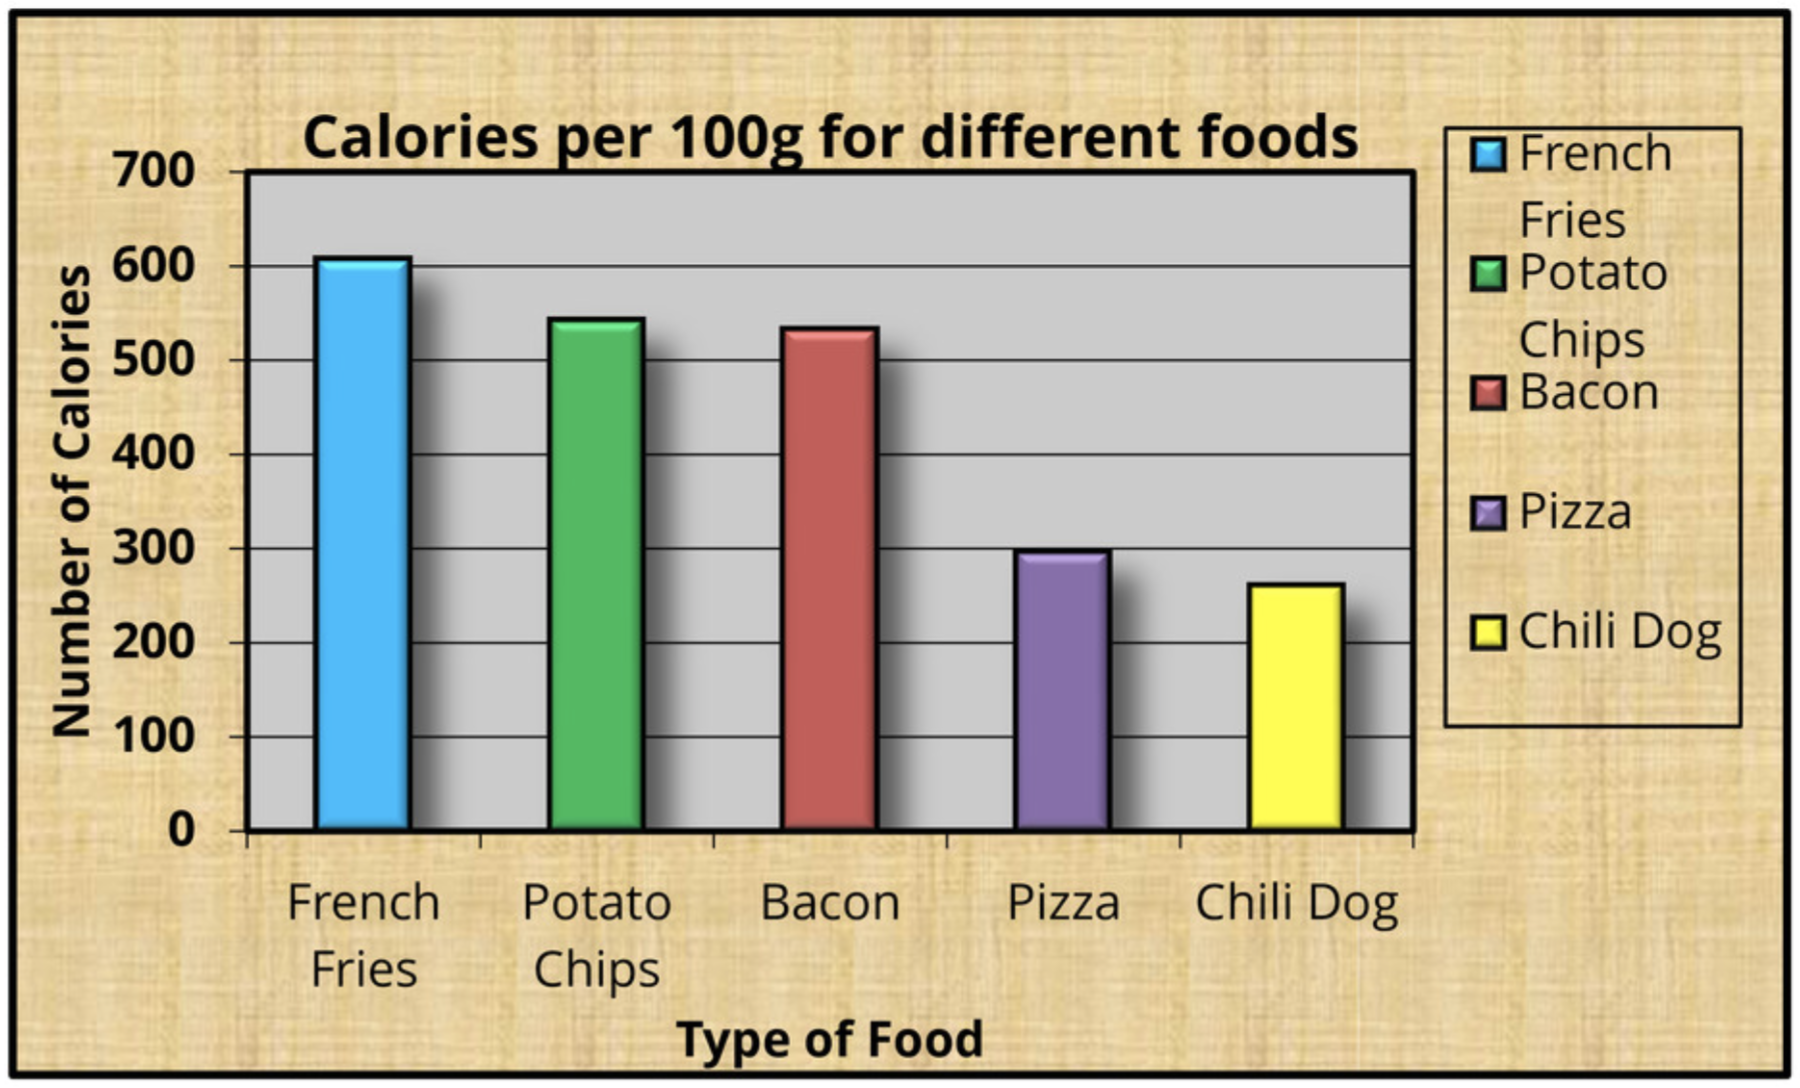
\includegraphics[width=\textwidth]{../figures/barplot-before}
% 	\caption{This is a fancy barplot.}
% 	\label{fig:barplot-before}
% \end{figure}

\newcommand{\image}[5][t]{
	\begin{figure}[#1]
		\centering
		\includegraphics[width=#2]{../figures/#3}
		\caption{#4}
		\label{fig:#5}
	\end{figure}
}

% Custom command to insert two images next to each other with a margin caption
% This command uses 6 required and one optional arguments/parameters with the following meaning:
%
% Optional:
% 1 - Position of the figure (the default position is 't' for top; if no argument is provided, 't' is used
%
% Required:
% 1 - Path to the frist image (inside the figures folder)
% 2 - Path to the second image (inside the figures folder)
% 3 - Caption of the image
% 4 - Label for the image (a universal fig: is prepended)
%
% Required --------------------------------------------------------------------------------------
% Optional -----------------|		  |			    |					|					    |
% 						    V		  V (1)		    V (2)				V (3)				    V (4)
% Example Usage: \twoimages[h]{barplot-before}{barplot-after}{This is a fancy barplot.}{barplot-sidebyside}
%
% The result will be the same as:
%
% \begin{figure}[h]
% 	\centering
% 	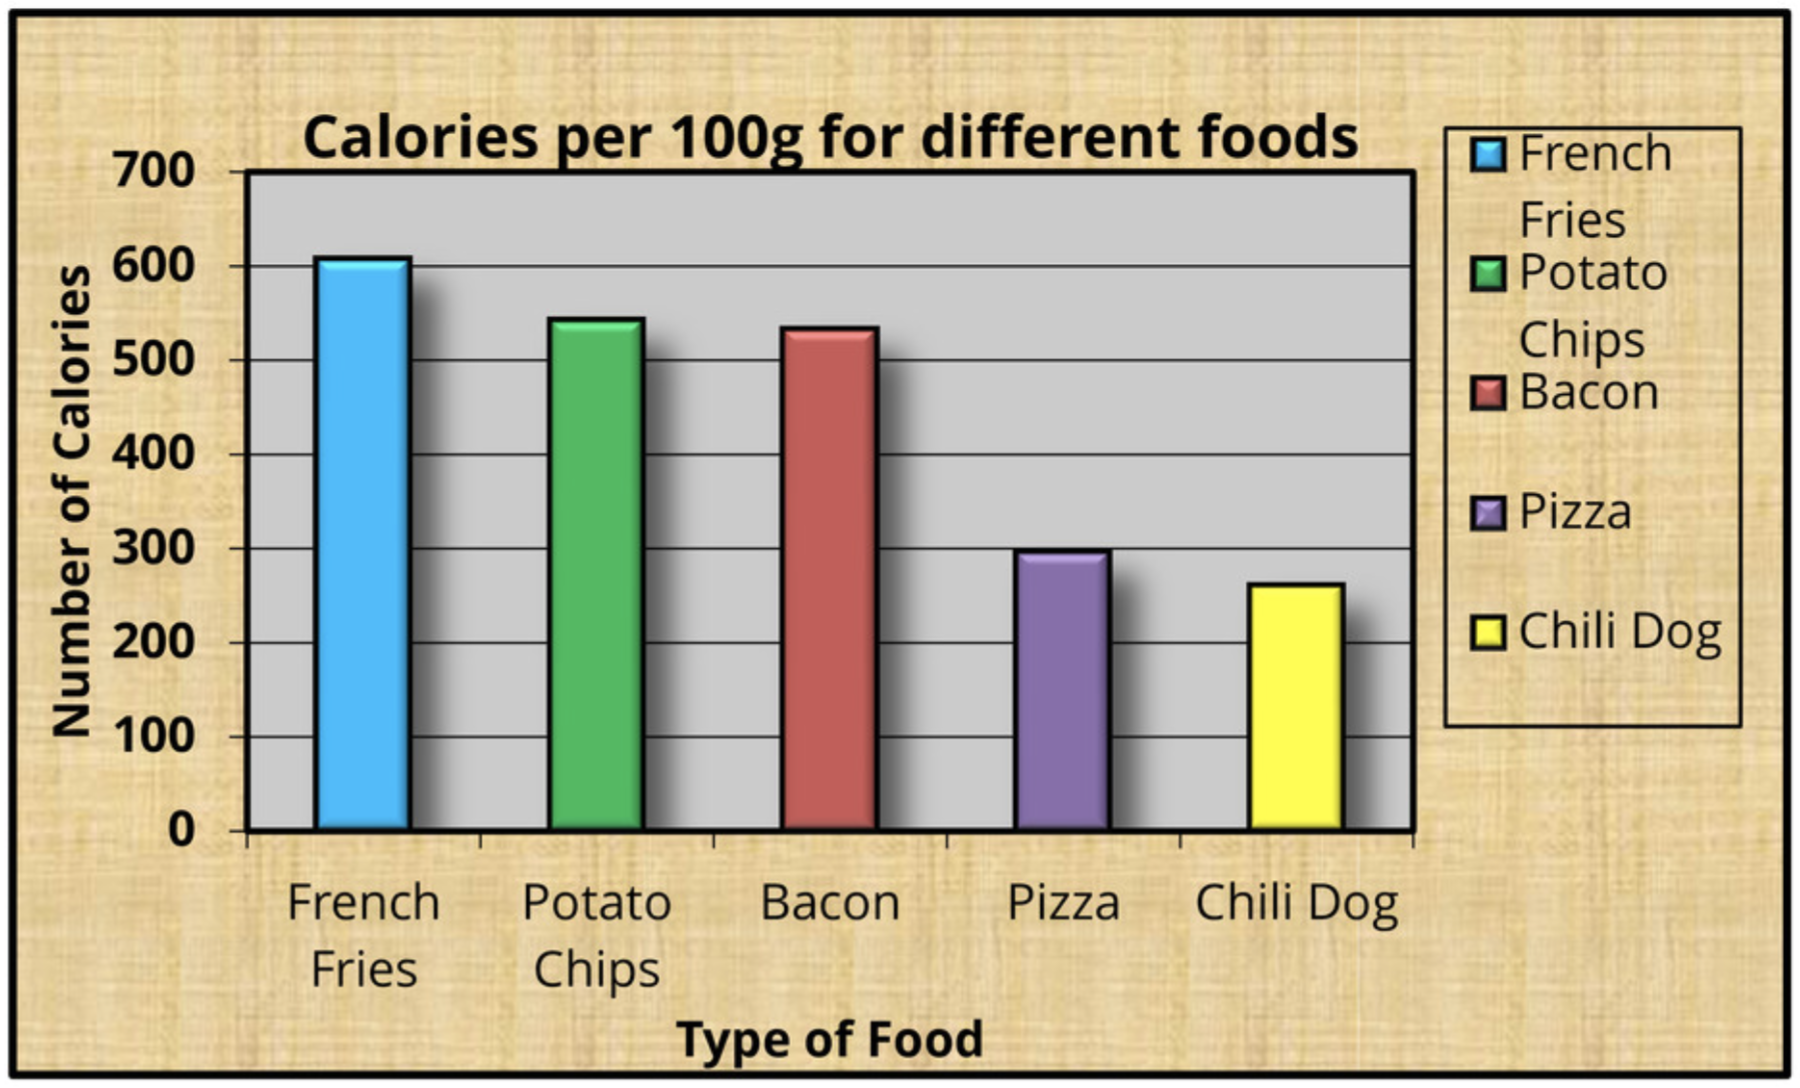
\includegraphics[width=0.48\textwidth]{../figures/barplot-before}
% 	\hspace{\fill}
% 	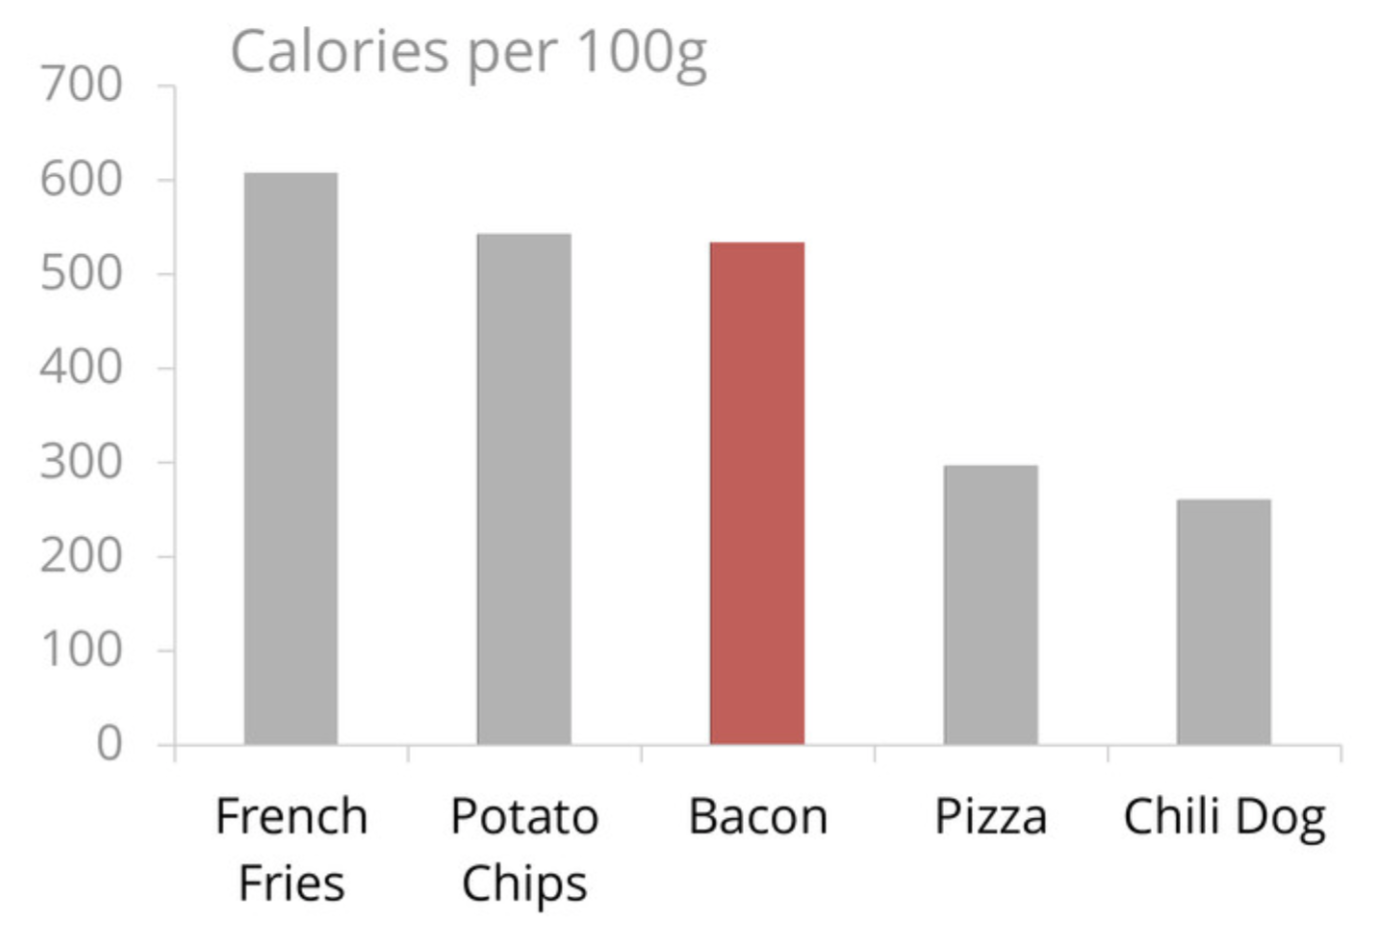
\includegraphics[width=0.48\textwidth]{../figures/barplot-after}
% 	\caption{\label{fig:barplot-sidebyside}This is a fancy barplot.}
% \end{figure}

\newcommand{\twoimages}[5][t]{
	\begin{figure}[#1]
		\centering
		\includegraphics[width=0.48\textwidth]{../figures/#2}
		\hspace{\fill}
		\includegraphics[width=0.48\textwidth]{../figures/#3}
		\sidecaption{\label{fig:#5}#4}[-2\baselineskip]
	\end{figure}
}


% Custom image command for wide figures
% This command uses 4 required and one optional arguments/parameters with the following meaning:
%
% Optional:
% 1 - Position of the figure (the default position is 't' for top; if no argument is provided, 't' is used
%
% Required:
% 1 - Path to the image (inside the figures folder)
% 2 - Caption of the image
% 3 - Label for the image (a universal fig: is prepended)
%
% Required ------------------------------------------------------------------
% Optional -----------------|		  |				 	 |					|
% 						    V		  V (1)		 	  	 V	(2)				V (3)
% Example Usage: \wideimage[h]{barplot-before}{This is a fancy barplot.}{barplot-before}
%
% The result will be the same as:
%
% \begin{figure*}[h]
% 	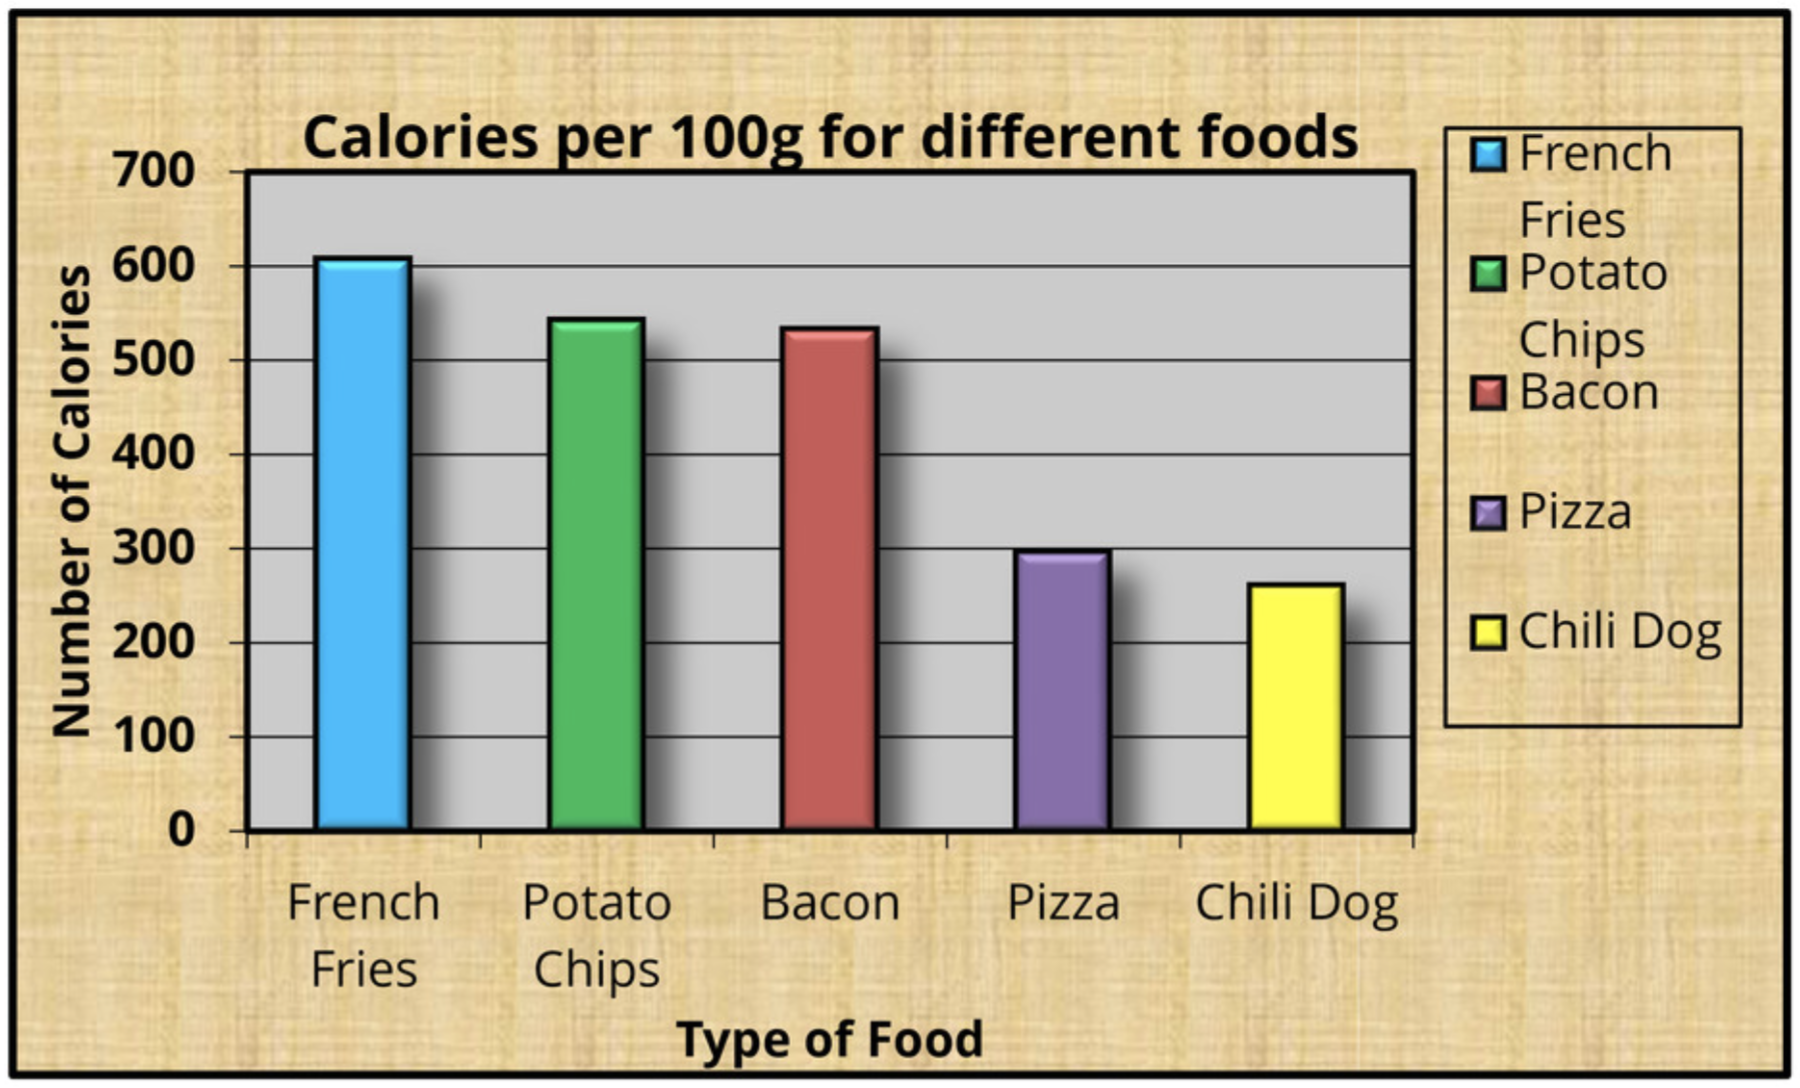
\includegraphics[width=\widefigurewidth]{../figures/barplot-before}
% 	\caption{This is a fancy barplot.}
% 	\label{fig:barplot-before}
% \end{figure*}
%
% %%%%%%%%%%%%%%%%%%%%%%%
% % 	ATTENTION		%
% %%%%%%%%%%%%%%%%%%%%%%%
% It seems this command messes with the position of other images, therefore it is advised to check the placement of other images.

\newcommand{\wideimage}[4][t]{
	\begin{figure*}[#1]
		\includegraphics[width=\widefigurewidth]{../figures/#2}
		\caption{\label{fig:#4}#3}
	\end{figure*}
}

% This command uses 3 required and one optional arguments/parameters with the following meaning:
%
% Optional:
% 1 - Vertical offset of the figure (the default offset is 1 for one line lower (negative numbers move the image up); if no argument is provided, 1 is used
%
% Required:
% 1 - Path to the image (inside the figures folder)
% 2 - Caption of the image
% 3 - Label for the image (a universal fig: is prepended)
%
% Required ----------------------------------------------------------------------
% Optional -------------------|			|				  |						|
% 							  V			V (1)			  V	(2)					V (3)
% Example Usage: \marginimage[2]{barplot-before}{This is a fancy barplot.}{barplot-before}
%
% The result will be the same as:
%
% \begin{marginfigure}[2\baselineskip]
% 	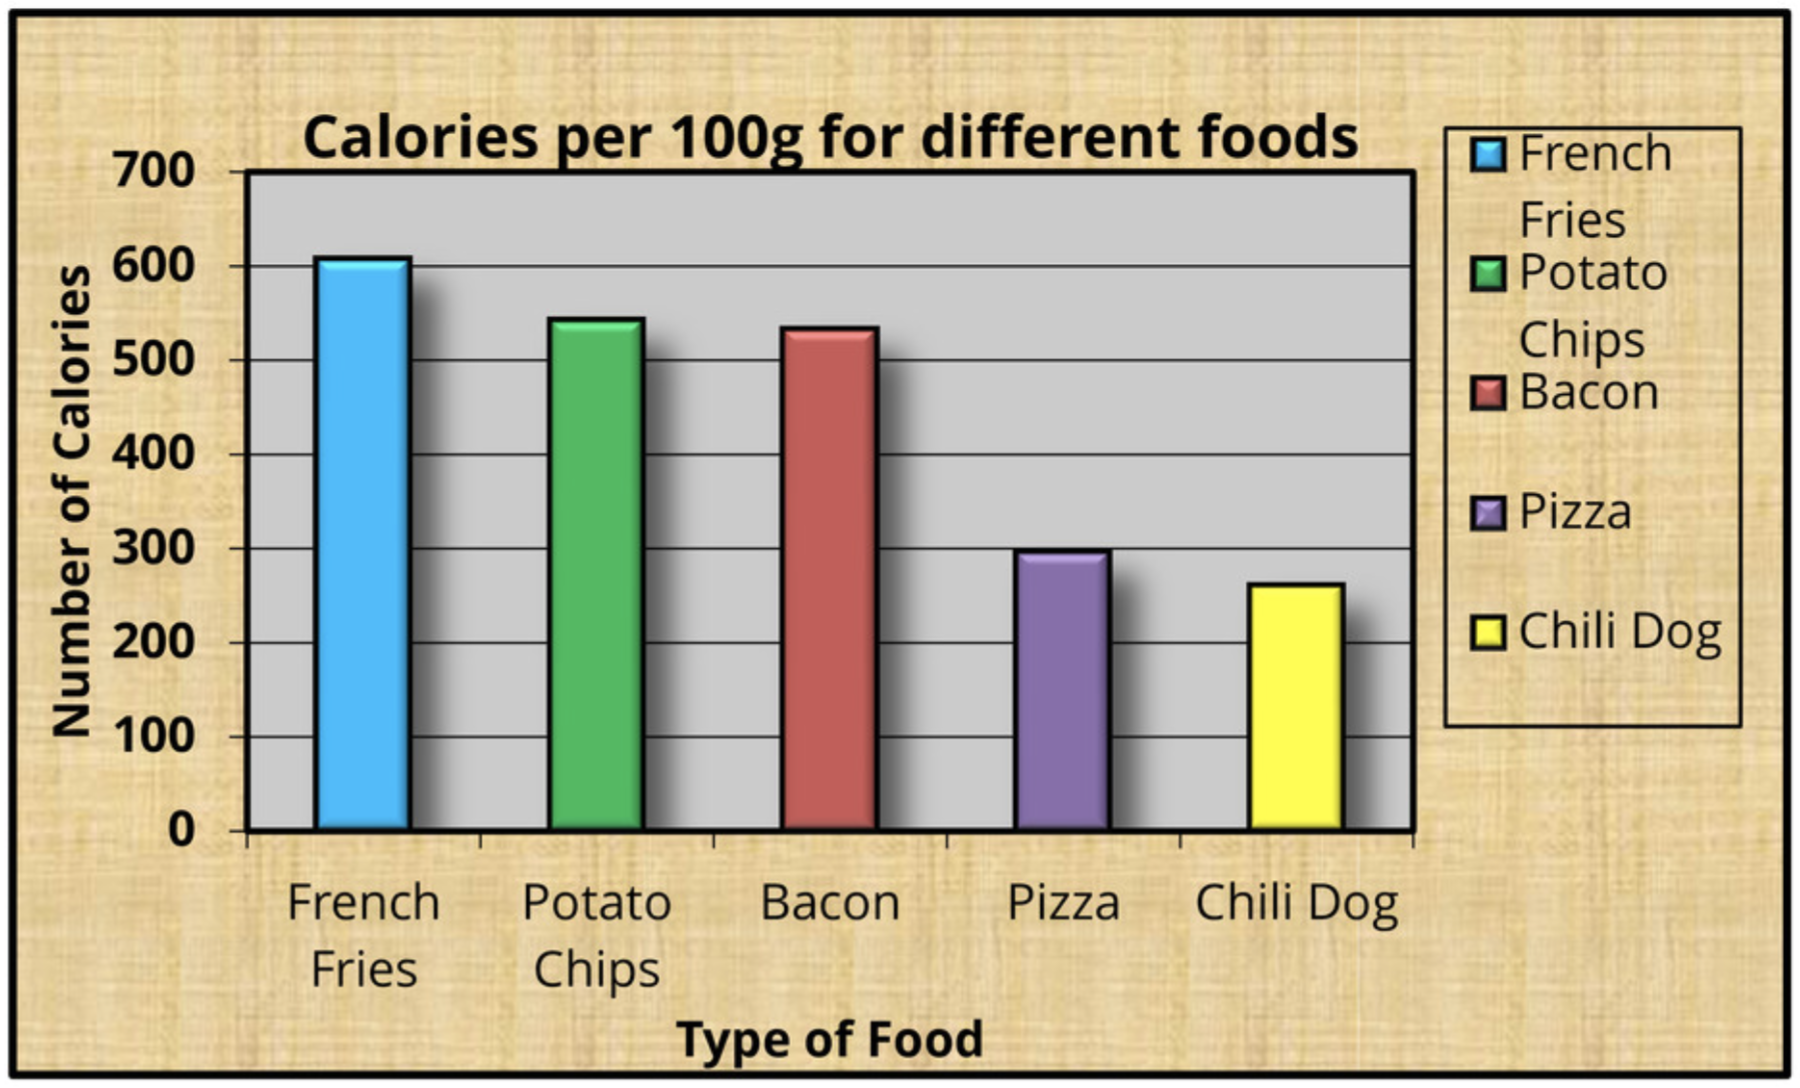
\includegraphics[width=\marginparwidth]{../figures/barplot-before}
% 	\caption{\label{fig:barplot-before}This is a fancy barplot.}
% \end{marginfigure}
\newcommand{\marginimage}[4][1]{
	\begin{marginfigure}[#1\baselineskip]
		\includegraphics[width=\marginparwidth]{../figures/#2}
		\caption{\label{fig:#4}#3}
	\end{marginfigure}
}
 % Load the custom commands from Misc/commands.tex

% Uncomment this command to make all links black:
%   useful for printing on black-white printers that do a
%   poor job at rasterizing colored text properly
%\hypersetup{colorlinks=false}
\addbibresource{clean-lit.bib} % The filename of the bibliography

\usepackage{bytefield}
\usepackage{calc}
%\usepackage{minted}

%----------------------------------------------------------------------------------------
%	THESIS INFORMATION
%----------------------------------------------------------------------------------------
\newcommand{\thesistype}{Bachelor} % type of your thesis (Bachelors, Masters, Doctoral ...)

%%% CHANGE THIS:
% Your thesis title, this is used in the title and abstract, print it elsewhere with \ttitle
\thesistitle{Alternative Approaches for Virtual Memory Management}

% date to be printed on the title, this will automatically update and be in the correct format
% If any changes to this format (Month JJJJ) are necessary the definition can be found in line 337
% of misc/setup.tex
\def\tdate{\monthyeardate\today}

%%% CHANGE THIS:
% Your name, this is used in the title page, print it elsewhere with \authorname
\author{Max Meidinger}

% Your supervisor's name, this is used in the title page, print it elsewhere with \supname
\supervisor{Prof. Dr. Michael Engel}

% Your university's name and URL, this is used in the title page, print it elsewhere with \univname
\university{\href{https://www.uni-bamberg.de/en/}{University of Bamberg}}

% Your research group's name and URL, this is used in the title page, print it elsewhere with \groupname
\group{\href{https://www.uni-bamberg.de/sysnap/}{Chair of Practical Computer Science, esp. Systems Programming}}

% Your department's name and URL, this is used in the title page, print it elsewhere with \deptname
\department{department not used}

% Your faculty's name and URL, this is used in the title page, print it elsewhere with \facname
% TODO: insert *your* degree program in the \faculty command below
% Applied Computer Science
% Computing in the Humanities
% Information Systems
% International Information Systems Management
% International Software Systems Science
% Software Systems Science
% Education in Business and Information Systems
\faculty{Software Systems Science Degree Program in the\\ \href{https://www.uni-bamberg.de/en/wiai/}{Faculty of Information Systems and Applied Computer Sciences}}

% Your address, this is not currently used anywhere in the template, print it elsewhere with \addressname
\addresses{address not used}

% Your subject area, this is not currently used anywhere in the template, print it elsewhere with \subjectname
\subject{subject not used}

% Keywords for your thesis, this is not currently used anywhere in the template, print it elsewhere with \keywordnames
\keywords{keywords not used}



% Stolen from https://tex.stackexchange.com/questions/105995/is-there-a-ready-solution-to-typeset-a-diff-file

\usepackage[svgnames]{xcolor}
  \definecolor{diffstart}{named}{Grey}
  \definecolor{diffincl}{named}{Green}
  \definecolor{diffrem}{named}{OrangeRed}

\usepackage{listings}
  \lstdefinelanguage{diff}{
    basicstyle=\ttfamily\small,
    morecomment=[f][\color{diffstart}]{@@},
    morecomment=[f][\color{diffincl}]{+\ },
    morecomment=[f][\color{diffrem}]{-\ },
  }


  % more piracy https://gist.github.com/AntonLydike/e339c3c3a4dcab8bc3c620b3fa436cda


% RISC-V Assembler syntax and style for latex lstlisting package
%
% These are risc-v commands as per our university (University Augsburg, Germany) guidelines.
%
% Author: Anton Lydike
%
% This code is in the public domain and free of licensing

% language definition
\lstdefinelanguage[RISC-V]{Assembler}
{
  alsoletter={.}, % allow dots in keywords
  alsodigit={0x}, % hex numbers are numbers too!
  morekeywords=[1]{ % instructions
    lb, lh, lw, lbu, lhu,
    sb, sh, sw,
    sll, slli, srl, srli, sra, srai,
    add, addi, sub, lui, auipc,
    xor, xori, or, ori, and, andi,
    slt, slti, sltu, sltiu,
    beq, bne, blt, bge, bltu, bgeu,
    j, jr, jal, jalr, ret,
    scall, break, nop
  },
  morekeywords=[2]{ % sections of our code and other directives
    .align, .ascii, .asciiz, .byte, .data, .double, .extern,
    .float, .globl, .half, .kdata, .ktext, .set, .space, .text, .word
  },
  morekeywords=[3]{ % registers
    zero, ra, sp, gp, tp, s0, fp,
    t0, t1, t2, t3, t4, t5, t6,
    s1, s2, s3, s4, s5, s6, s7, s8, s9, s10, s11,
    a0, a1, a2, a3, a4, a5, a6, a7,
    ft0, ft1, ft2, ft3, ft4, ft5, ft6, ft7,
    fs0, fs1, fs2, fs3, fs4, fs5, fs6, fs7, fs8, fs9, fs10, fs11,
    fa0, fa1, fa2, fa3, fa4, fa5, fa6, fa7
  },
  morecomment=[l]{;},   % mark ; as line comment start
  morecomment=[l]{\#},  % as well as # (even though it is unconventional)
  morestring=[b]",      % mark " as string start/end
  morestring=[b]'       % also mark ' as string start/end
}

% usage example:

% define some basic colors
\definecolor{mauve}{rgb}{0.58,0,0.82}

\lstset{
  % listings sonderzeichen (for german weirdness)
  literate={ö}{{\"o}}1
           {ä}{{\"a}}1
           {ü}{{\"u}}1,
  basicstyle=\tiny\ttfamily,                    % very small code
  breaklines=true,                              % break long lines
  commentstyle=\itshape\color{green!50!black},  % comments are green
  keywordstyle=[1]\color{blue!80!black},        % instructions are blue
  keywordstyle=[2]\color{orange!80!black},      % sections/other directives are orange
  keywordstyle=[3]\color{red!50!black},         % registers are red
  stringstyle=\color{mauve},                    % strings are from the telekom
  identifierstyle=\color{teal},                 % user declared addresses are teal
  frame=l,                                      % black line on the left side of code
  language=[RISC-V]Assembler,                   % all code is RISC-V
  tabsize=4,                                    % indent tabs with 4 spaces
  showstringspaces=false                        % do not replace spaces with weird underlines
}

% EOP - End of piracy
%----------------------------------------------------------------------------------------
%	END OF THESIS INFORMATION
%----------------------------------------------------------------------------------------

%\setcounter{tocdepth}{3}

\begin{document}

\selectlanguage{english}

\frenchspacing % do not add additional hspace after end of sentence full stop dot.

\frontmatter % Uses roman page numbering style (i, ii, iii, iv...) for the pre-content pages

\hypersetup{urlcolor=black}

%%%%%%%%%%%%%%%%%%%%%%%%%%%%%%%%%%%%%%%%%%%%%%%%%%%
%
% File: titlepage.tex
%
% This file is part of the PSIThesis.cls
% LaTeX documentclass
%
% The code in this file is made available
% under the following license:
%
% LPPL v1.3c (http://www.latex-project.org/lppl)
%
%%%%%%%%%%%%%%%%%%%%%%%%%%%%%%%%%%%%%%%%%%%%%%%%%%%


\pagestyle{plain} % Default to the plain heading style until the thesis style is called for the body content

%----------------------------------------------------------------------------------------
%	TITLE PAGE
%----------------------------------------------------------------------------------------

\begin{titlepage}

	\newgeometry{
		inner=4cm, % Inner margin
		outer=4cm, % Outer margin
		marginparwidth=0cm,
		marginparsep=0mm,
		bindingoffset=.5cm, % Binding offset
		top=2.5cm, % Top margin
		bottom=2.5cm, % Bottom margin
		showframe % Uncomment to show how the type block is set on the page
	}

	\begin{center}

		\vspace*{.06\textheight}

		% The logo of University of Bamberg. Do not use the logo without permission.
		% Using it on the title page of a thesis is acceptable.
		% TODO Add your own logo here. Do yourself and your readers a favor and use
		%      a vectorized logo (PDF) instead of a bitmap (PNG, JPEG)
		
\includegraphics[width=35mm]{misc/UB_Logo_20mm_CMYK.pdf}

		\vspace*{.06\textheight}

		{\LARGE \textls[130]{\MakeUppercase{\univname}}\par}\vspace{2\baselineskip} % University name

		% TODO uncomment the next line when you write a thesis to display the supervisor
		%{\large \facname}
		% TODO comment out the next line when you write a thesis
		{\large ~} % For use in the guide

		\vspace{1.5cm}

		% TODO uncomment the next line when you write a thesis to display the supervisor
		%\textsc{\Large \thesistype 's~Thesis}\\[1cm] % For use in the thesis
		% TODO comment out the next line when you write a thesis
		\textsc{\Large ~}\\[1cm] % For use in the guide

		%\HRule \\[0.4cm] % Horizontal line
		%
		{\huge \bfseries \ttitle\par}\vspace{1cm} % Thesis title

		%\HRule \\[1.5cm] % Horizontal line


		\textsc{\Large by}\\[1cm]

		{\Large \authorname}

		\vspace{1.5cm}

		% TODO uncomment the next two lines when you write a thesis to display the supervisor
		\emph{Supervisor:} \\
		\supname\\[1cm]
		%%

		\groupname%\\[2cm] % Research group name and department name

		\vfill

		{\large \tdate} % Date

		% TODO remove the following lines when you write a thesis
		% \vspace{0.25ex}

		% {\small \tversion}

		% \vspace{0.25ex}

		% {\small Links to this document:}\\
		% {\small \url{\doiurl}} (initial version)\\
		% {\small \url{\githuburl} (most recent version)}
		% Remove lines up to this line

		\vfill
	\end{center}

	\restoregeometry

\end{titlepage}


 % Typeset the titlepage

\hypersetup{urlcolor=ubblue80}


%----------------------------------------------------------------------------------------
%	QUOTATION
%----------------------------------------------------------------------------------------

% \vspace*{0.2\textheight}

% \noindent\enquote{\itshape Thanks to my solid academic training, today I can write hundreds of words on virtually any topic without possessing a shred of information, which is how I got a good job in journalism.}\bigbreak

% \hfill Dave Barry


%----------------------------------------------------------------------------------------
%	ABSTRACT PAGE
%----------------------------------------------------------------------------------------

\begin{abstract}
  \emph{Virtual memory} (VM) is a fundamental component of modern computer systems, widely adopted across various computing environments, from embedded devices to large-scale data centers. While it initially served to automate memory management by transparently swapping pages between main memory and secondary storage, it now plays a crucial role in ensuring system security, process isolation, and overall flexibility. However, the increasing overhead associated with traditional VM systems — originally designed for resource-constrained environments — has led to performance bottlenecks, particularly in systems with high memory demands and applications with poor spatial locality. The ever-increasing depth of conventional hierarchical page tables further exacerbates these challenges.

  To address these limitations, alternative approaches like \emph{Inverted Page Tables} are used, but they have their own set of downsides. The plethora of designs and approaches to optimizing these designs suggest general performance problems. This thesis proposes an approach that aims to eliminate the need for page tables and main memory accesses altogether by using specialized mapping functions instead of costly page table walks. These mappings promise faster address translation, as they omit the cost associated with the page table accesses, while providing flexibility to system designers by defining them in software. This allows tailoring the virtual memory system to specific use cases.

  The thesis details the theoretical foundations and practical implementation of a platform designed to facilitate the exploration and experimentation with such mapping functions. It also presents an initial simplified VM system prototype that demonstrates the feasibility of the approach.
\end{abstract}


%----------------------------------------------------------------------------------------
%	ACKNOWLEDGEMENTS
%----------------------------------------------------------------------------------------

%\begin{acknowledgements}
% %\addchaptertocentry{\acknowledgementname}
% Add the acknowledgements to the table of contents (not recommended)
%
%The acknowledgments and the people to thank go here.
%\end{acknowledgements}


%----------------------------------------------------------------------------------------
%	TABLE OF CONTENTS
%----------------------------------------------------------------------------------------

\cleardoublepage

% Table of Contents uses a wider layout than the main content
\newgeometry{
  head=13.6pt,
  top=27.4mm,
  bottom=27.4mm,
  inner=24.8mm,
  outer=24.8mm,
  marginparsep=0mm,
  marginparwidth=0mm,
}
{
  \hypersetup{linkcolor=black}
  \tableofcontents % Prints the ToC entries
}
\restoregeometry

%----------------------------------------------------------------------------------------
%	DEDICATION
%----------------------------------------------------------------------------------------

% \dedicatory{For/Dedicated to/To my\ldots}


%----------------------------------------------------------------------------------------
%	THESIS CONTENT - CHAPTERS
%----------------------------------------------------------------------------------------
\mainmatter % From here on, numeric (1,2,3...) page numbering
\pagestyle{thesis} % Return the page headers back to the "thesis" style

% Define some commands to keep the formatting separated from the content
\newcommand{\keyword}[1]{\textbf{#1}}
\newcommand{\tabhead}[1]{\textbf{#1}}
\newcommand{\code}[1]{\texttt{#1}}
\newcommand{\file}[1]{\texttt{#1}}
\newcommand{\option}[1]{\texttt{\itshape#1}}

% Figures will automatically be searched for in the Figures subdirectory
\graphicspath{{./figures/}{./examples/}}

%%% CHANGES NEEDED HERE
%
% Include the chapters of the thesis as separate files from the Chapters folder
% Uncomment the lines as you write the chapters
% Mind the \input instead of the \include here, that change is necessary for the appendix formatting
% Due to the \input command you also need to provide the .tex file ending



\chapter{Introduction} % Main chapter title
% TODO CHECK 2-3 Seiten
% TODO CHECK Keine Ergebnisse
% TODO CHECK Keine Definitionen
% TODO CHECK Alles relevante vorhanden



% -------------------------------------------------------------------------------------------------
%                                             Structure
% -------------------------------------------------------------------------------------------------



% Motivation for VM
% Importance of vm
% Functional requirements
% Description of Problems with VM
% Unclear interfaces
% Performance -> Applications with poor spatial locality
% Description of Approach

% Proof of concept
% Description of Contents









% -------------------------------------------------------------------------------------------------
% -------------------------------------------------------------------------------------------------
% -------------------------------------------------------------------------------------------------
% -------------------------------------------------------------------------------------------------
% Motivation
% Most Computer use Virtual Memory

% THIS SECTION may primarily be about some facts about VM

\textbf{Virtual memory} provides a multitude of features that vastly simplify the life of application programmers \cite{jacob1998virtualissues}. Computer systems of all scales, ranging from small embedded devices to huge data centers use virtual memory \cite{bhattacharjee2017architectural}.
While originally being used to automate the task of swapping pages of processes between main memory and secondary storage transparently to the processes \cite{jacob1998virtualissues}, it now is the foundation for security, reliability, process isolation and flexibility \cite{wales1999virtual,jacobVirtualMemoryContemporary1998}.

With ever increasing memory sizes of systems and memory requirements of applications, the \textbf{overhead} of virtual memory systems, being developed for systems that only had scarce resources available \cite{halbuer2023morsels}, is degrading performance and increase power consumption significantly \cite{zagieboylo2020cost}.
Orthodox hierarchical page table organizations \cite{tanenbaumOS} can get as deep as 5 levels in commodity hardware \cite{intel5LevelPaging5Level2017}. Not only does this add a level of indirection for each page table walk, this penalty is even higher in virtualized systems, potentially accounting for up to 5\% - 90\% of the runtime \cite{yaniv2016hash}.

\textbf{Alternative designs} like inverted page tables realize page table mappings using hash functions \cite{tanenbaumOS}. While reducing the number of additional memory references, these approaches have problems on their own: Some features of virtual memory systems become harder to implement, exacting additional performance penalties \cite{yaniv2016hash} and page table lookups can get a lot more expense when following collision chains \cite{jacob1998look}.

Chapter \ref{chap:related} will show, that there are a lot of different \textbf{approaches to optimize} the virtual memory system.
This shows that there is little agreement on how the virtual memory system is best implemented \cite{jacob1998look}.
However, most of the optimization approaches still relied on page table structures to do the bookkeeping of the mappings.

\textbf{This thesis} explores the idea of getting rid of page table structures all together and base the mapping of virtual to physical addresses on specially crafted functions (for example non-cryptographic hash functions \cite{mittelbach2021non}).
Hash functions implemented by simple arithmetic instructions are orders of magnitude faster than the multiple memory accesses required by a page table walk \cite{tanenbaumOS} and allowing them to be defined in software gives the operating system a lot of flexibility to fit the implementation of the mapping function to the custom needs of the use case.

This thesis will describe the \textbf{theory and implementation} of a platform that facilitates the definition and the experimentation with such mapping functions and also shows a first simple mapping function that realizes a simplified virtual memory system without any page tables.


% Inhaltsbeschreibung
\textbf{Chapter 2} provides an overview of the fundamentals of virtual memory systems, software-managed virtual memory systems and some basics of the virtual memory system of the RISC-V ISA.

\textbf{Chapter 3} takes a look at previous work that also approaches the topic of optimizing virtual memory systems.

\textbf{Chapter 4} describes the theoretical development of the idea presented in this paper and thus provides the foundation for the implementation.

\textbf{Chapter 5} describes the implementation. It delves into the specifics of the programming platforms and outlines the implementation process step by step. This chapter also includes an overview of the debugging techniques used for verification and troubleshooting of the implementation.

\textbf{Chapter 6} critically examines the current state of the theoretical development and implementation, analyzing the results in light of typical requirements for other virtual memory systems. It also includes a discussion on further deepening the approach.

% In \textbf{Chapter 7}, suggestions are made for future work building upon this thesis. These suggestions refer to previously excluded topics, such as hardware optimizations of the idea.



% -------------------------------------------------------------------------------------------------







% -------------------------------------------------------------------------------------------------
% -------------------------------------------------------------------------------------------------
% -------------------------------------------------------------------------------------------------
% -------------------------------------------------------------------------------------------------

\chapter{Fundamentals} % Main chapter title

\label{chap:fund}
% \section{Virtual Memory}
% Grundlagen auffrischen, kurz die Motivation und Grundkonzepte von Virtual Memory erläutern
% Da eventuell kurz auf Atlas eingehen und wie sehr sich VM bis jetzt entwickelt hat
% Quellen:
% - Lehrbücher: VM Definitionen und Übersichtsbeschreibungen
% - Architectural and operating system support for virtual memory

% VM Properties and benefits:
- idealized abstraction of storage resources available on a machine
- virtual to physical mapping
- flexibility to place actual data anywhere on the available disk
- emulate bigger memory than actually available
- foundation for isolation/security
- Implement flexible paging the swap pages between main memory and secondary storage

% \subsection{What is Virtual Memory}


% Purpose of Section:
% Ziegen, dass es keinen Standard gibt und es viele Verschiedne Möglichkeiten gibt um VM zu realisieren
% Quellen:
% [ A look at several...]
% [ Issues of implementation]
% \section{Implementation of Virtual Memory Systems}
% \subsection{ Overview of different implementations (Inverted/Hierarchical/Multi-Level)}
% \subsection{ Comparison of differnt implementations with regards to performance and features like page sharing}

% \section{Hardware support}
% \subsection{MMU & TLB}
% \subsection{HW-Dependent PTE Structure}
% \subsection{A typical Page Table Walk}

% \section{ Sofware Paging approaches}
% \subsection{More flexibilty}

\todo{general motivation of virtual memory and what it provides}
\todo{then a discussion on typical virtual memory systems and their trade offs}
% related work will then come in to discuss approaches close to my approach
\begin{figure*}[t]
    \centering
    \begin{bytefield}[bitwidth=\widefigurewidth/39,bitheight=\widthof{~PBMT~}, bitformatting={\tiny\bfseries}, boxformatting={\centering}]{39}
        \bitheader[endianness=big]{38,30,29,21,20,12,11,0} \\
        \bitbox{9}{VPN[2]} &
        \bitbox{9}{VPN[1]} &
        \bitbox{9}{VPN[0]} &
        \bitbox{12}{Page Offset}\\
    \end{bytefield}
    \caption[RISC-V Sv39 Virtual Address]{RISC-V Sv39 Virtual Address}
    \label{fig:fundamentals:sv39va}
\end{figure*}

\begin{figure*}[t]
    \centering
    \begin{bytefield}[bitwidth=\widefigurewidth/56,bitheight=\widthof{~PBMT~}, bitformatting={\tiny\bfseries}, boxformatting={\centering}]{56}
        \bitheader[endianness=big]{55,30,29,21,20,12,11,0} \\
        \bitbox{26}{PPN[2]} &
        \bitbox{9}{PPN[1]} &
        \bitbox{9}{PPN[0]} &
        \bitbox{12}{Page Offset}\\
    \end{bytefield}
    \caption[RISC-V Sv39 Physical Address]{RISC-V Sv39 Physical Address}
    \label{fig:fundamentals:sv39pa}
\end{figure*}

\begin{figure*}[t]
    \centering
    \begin{bytefield}[bitwidth=\widefigurewidth/64,bitheight=\widthof{~PBMT~}, bitformatting={\tiny\bfseries}, boxformatting={\centering}]{64}
        \bitheader[endianness=big]{63,62,61,60,54,53,28,27,19,18,10,9,8,7,6,5,4,3,2,1,0} \\
        \bitbox{1}{N} &
        \bitbox{2}{\rotatebox{90}{PBMT}} &
        \bitbox{7}{Reserved} &
        \bitbox{26}{PPN[2]} &
        \bitbox{9}{PPN[1]} &
        \bitbox{9}{PPN[0]} &
        \bitbox{2}{\rotatebox{90}{RSW}} &
        \bitbox{1}{D} &
        \bitbox{1}{A} &
        \bitbox{1}{G} &
        \bitbox{1}{U} &
        \bitbox{1}{X} &
        \bitbox{1}{W} &
        \bitbox{1}{R} &
        \bitbox{1}{V}
    \end{bytefield}
    \caption[RISC-V Sv39 Page Table Entry]{RISC-V Sv39 Page Table Entry}
    \label{fig:fundamentals:sv39pte}
\end{figure*}


\begin{figure*}[t]
    \centering
    \begin{bytefield}[bitwidth=\widefigurewidth/64,bitheight=\widthof{~PBMT~}, bitformatting={\tiny\bfseries}, boxformatting={\centering}]{64}
        \bitheader[endianness=big]{63,60,59,44,43,0} \\
        \bitbox{4}{Mode} &
        \bitbox{16}{ASID} &
        \bitbox{44}{PPN} \\
    \end{bytefield}
    \caption[RISC-V Sv39 \texttt{satp} CSR]{RISC-V Sv39 \texttt{satp} CSR}
    \label{fig:fundamentals:sv39satp}
\end{figure*}

\begin{figure*}[ht!]
    \centering
    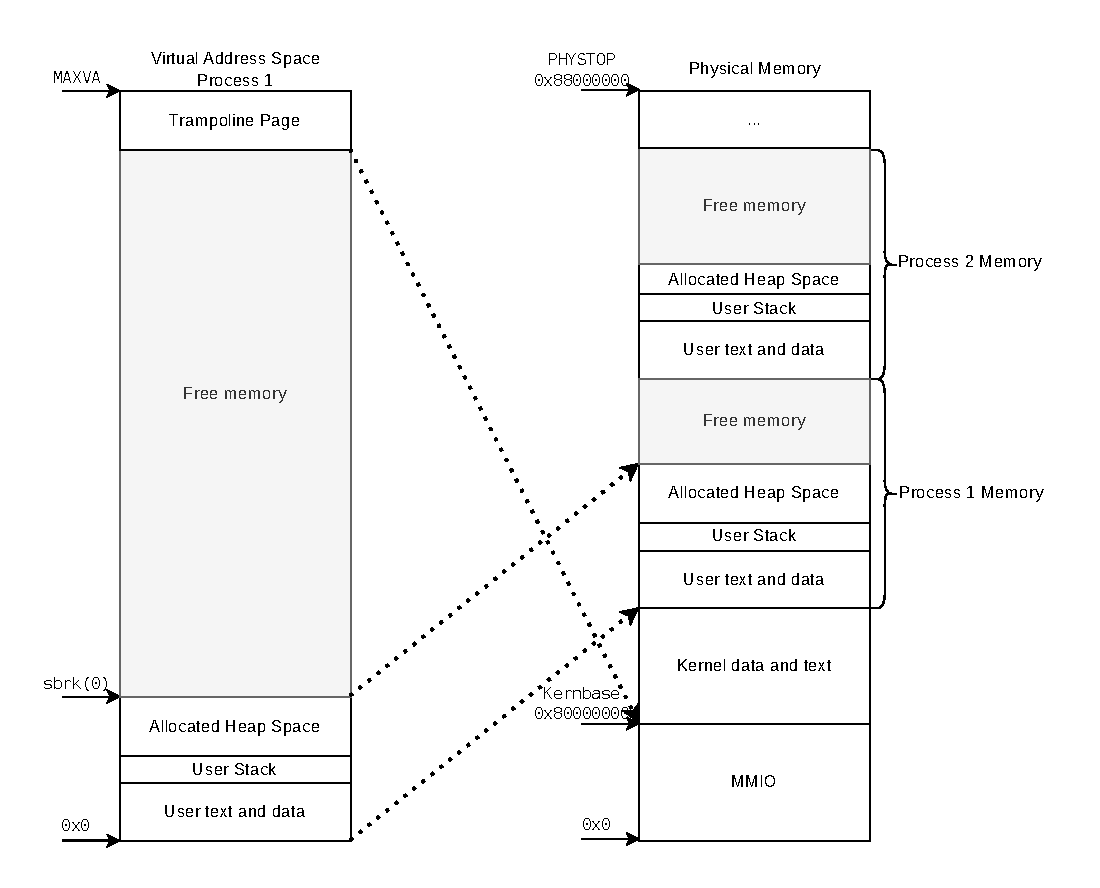
\includegraphics[]{figures/simple_mapping.pdf}

    \caption[Simple Mapping Scheme]{Simple Mapping Scheme}
    \label{fig:theory:simplemapping}
\end{figure*}

%RISCV - VM - PTE bits, Global bits

\section{Programming Platform}
\subsection{Qemu}
\subsection{xv6 RISC-V}
\chapter{Related Work}

\label{chap:related}
This work can be broadly classified to be in the field of Virtual Memory optimization. There is a large body of literature that deals with optimizing the Virtual Memory system, as it lies on the critical path of every memory operation.

There are different approaches or perspectives to addressing the system (this is not an exhaustive list):

\begin{itemize}
    \item page table structures and their optimization, e.g., inverted or hierarchical
    \item caching of pages, PTEs in the TLB, and cache indexing
    \item cache replacement strategies
    \item cache sizes, associativity of caches
    \item Page Walk Caches (PWCs) to store partial translation results
\end{itemize}


% -------------------------------------------------------------------------------------------------

% Guarded Page Tables
\textbf{\cite{liedtkeGPT}} shows an innovative design leveraging the flexibility of software-managed
address translation.
The design of Guarded Page Tables (GPTs) is based on hierarchical page tables, but allows skipping over levels of the table to reach translation results faster.
This proves to be very effective for increasing the performance of virtual memory systems, as the biggest penalty comes from page tables walks needing to reference memory for every level in the page table.
Gernot Heiser showcases a practical implementation of GPTs in the L4/MIPS system \cite{heiserAnatomyHighPerformanceMicrokernel}.



% -------------------------------------------------------------------------------------------------

% In Cache Software Managed Address Translation
\textbf{\cite{jacobSoftwaremanagedAddressTranslation1997}} explores software-managed address translation and analyses the efficiency of a PowerPC implementation
of the presented design they call \textit{softvm}. They show that
software-managed address translation can achieve better performance and
at the same time simplify hardware by dispensing with translation caches and
the hardware state-machine for walking the page table.
The approach is based on handling virtually indexed and tagged cache misses in
software.
With sufficiently sized virtual caches the system can go for long periods
without requiring translations.
Not unlike this paper, they extend the PowerPC architecture by two new instructions
to write entries to the cache. However, their design uses software page table
walks to find translations on cache-miss, while the approach presented in this
paper presents a software-based TLB fill mechanism with segmented
memory allocation.
% TODO Further elaboration on the Background chapter of jacobSoftwaremanagedAddressTranslation1997

% -------------------------------------------------------------------------------------------------

% Translation Caching skip dont walk -> Translation Caches
\textbf{\cite{barrTranslationCachingSkip}} examines the design space of translation caches in MMUs. These caches are not the same as TLBs: TLBs contain full translation results, while the translation caches considered here contain partial translations. In the case of a cache hit, these partial translations allow the system to skip individual steps when traversing the page table tree, thereby saving one or more memory accesses. Otherwise, each level of translation requires a memory reference. These caches are also referred to as Page Walk Caches (PWC) \cite{yaniv2016hash}.

The specific translation cache designs of AMD and Intel platforms are examined and compared to three other designs proposed by the authors. Barr et al. conclude that radix page tables, by caching entries at higher page table levels, can outperform inverted page table designs.

This work focuses on optimizing the memory path by eliminating page tables and using a software-controlled TLB, and it does not further consider caches aside from the TLB.



% -------------------------------------------------------------------------------------------------

% Hash don't Cache
\textbf{\cite{yaniv2016hash}} challenges the results of \cite{barrTranslationCachingSkip} and argues that the obtained results are based on a suboptimal implementation of the inverted page table.

They conclude that a well-optimized inverted page table can outperform a radix page table equipped with PWCs. However, they also address the conceptual disadvantages of inverted page tables. For example, it is more difficult to implement superpages.

The work takes a closer look at the differences between various page table designs and the requirements of a memory system (such as superpages or page sharing). These requirements are also important for the design presented here. However, this work aims to avoid using page table structures altogether.


% -------------------------------------------------------------------------------------------------

% Every walk’s a hit: making page walks single-access cache hits
\textbf{\cite{park2022every}} identifies that today’s memory capacities far exceed the coverage of TLBs, causing memory-hungry applications to suffer from frequent page table walks (PTWs).

Two approaches are presented to reduce the associated costs: The first approach aims to reduce the number of memory references per PTW by combining two levels of the page table into one. The second approach modifies the cache replacement policy so that cache entries containing PTEs are more likely to remain in the cache during periods with many TLB misses, allowing PTWs to run directly from the cache instead of being loaded from main memory.

They show a 2.3\% performance improvement from flattening the page table tree, 6.2\% through cache prioritization, and a combined performance improvement of 9.2\%. Both approaches focus on optimizing access to page table structures and are separate from this work, as this work aims to eliminate these structures entirely.


% -------------------------------------------------------------------------------------------------

% Elastic Cuckoo Page Table
\textbf{\cite{skarlatos2020elastic}} presents a novel page table design called \textit{Elastic Cuckoo Page Tables}. The design exploits memory-level parallelism to enable fully parallel page table lookups. At the core of the design is the Elastic Cuckoo Hashing algorithm, which allows multiple hashing locations for a given element and enables efficient, gradual resizing of the hash table. Skarlatos et al. demonstrate an application execution speedup of 3-18\% using the Elastic Cuckoo Page Table design.



% -------------------------------------------------------------------------------------------------

\cite{zagieboylo2020cost} proposes an approach that shifts responsibilities of memory management in
parts back to the applications: All applications get a fixed-size chunks of physical memory and then have to manage allocations across these blocks.
Thus, the task of memory management with the chunks falls to compilers, language runtimes and the applications themselves.
This approach does not require any address translation and thus gets completely rid of the overhead associated with the virtual memory system.
Common features of virtual memory, like memory space protection can still be implemented with physical memory protection mechanisms present on commodity hardware.
Overall, this approach trades a reduction for complexity of the hardware with increased complexity on the software side.

The design presented in this paper resorts to bigger segments per process, but generally aims to keep the memory management responsibilities with the operating system. It tries to get rid of the page table structure in favor of mapping functions.

% -------------------------------------------------------------------------------------------------

\cite{halbuer2023morsels} argues that prevailing memory management system designs are becoming increasingly inefficient given modern systems that have very big main memories and workloads that require large in-memory data sets.
The paper presents a novel approach addressing the limitations of current methods with \emph{Morsels}.
These Morsels are self-contained memory object, spanning entire page table sub-trees, thus allowing efficient remapping, sharing and reducing memory overhead.
They reuse existing interfaces and work on top of existing page table structures to provide a supplementary layer to improve the efficiency of memory-intensive applications.

% -------------------------------------------------------------------------------------------------

The related work presented here focuses on optimizing current page table designs and their hardware
support. This work will explore the feasibility of implementing virtual memory without any page table whatsoever using a specialized mapping function to generate virtual to physical mappings.
This promises to reduce the overhead of TLB misses caused by expensive main memory access.


\chapter{Theory}
\label{chap:theory}

% -------------------------------------------------------------------------------------------------
%                                            Structure
% -------------------------------------------------------------------------------------------------

% - Reiteration of Idea       -> Was wird hier gemacht    -> Was benötigt man dafür

% - Impl Platform             -> Was provided die Hardware und Plattform schon, Was braucht es noch?

% - Implementation Steps      -> Overview over the implementation chapter (but without the single address cases)

% -Übersicht über die benötigten Änderungen
%     - TLB Miss Exception
%         - Exceptions and TLBS in RISC-V
%         - New Exception
%         - Vorlage: MIPS
%             - Riscv Exception basics (if not in fundamentals)
%             - New Exceptions? -> Was man beachten muss


%      - Exception Handler in general
%             - General Stuff, xv6 Exception Handler
%             - Vectored 
%             - All registers that come into play
%             - xv6 book, exception machinery

%         - Exception Handler for the TLB Miss exception

%     - TLB Filling
%         - Vorlage MIPS

%         - RISCV CSRs -> Extensibility


%         - QEMU TLB


%         - Concrete CSRs for TLB filling (THIS IS THE RESULT OF THIS CHAPTER)
%             (- TLB Flushing, Replacement policy (vs mips))


%     - Mapping functions
%         - Segmented
%         - More?







% -------------------------------------------------------------------------------------------------
%                                            Intro
% -------------------------------------------------------------------------------------------------
% Überblick über die Idee schaffen -> Virtueller Speicher durch funktion möglich


This chapter presents the theoretical foundation of the the implementation presented in the next chapter.
It will start with a short elaboration on the general idea followed by a description of the
programming platform.\\
It then presents the theory behind the different components of the implementation.
% Then?

% -------------------------------------------------------------------------------------------------
%                                            Idea
% -------------------------------------------------------------------------------------------------
% Beantwortet die Frage: Was wird hier überhaupt gemacht? (Ohne zu sehr ins detail zu gehen)
% Auch die Motivation und was das Ergebnis sein könnte/ erwartet ist



% Conclusion on previous Work -> Still need a memory access

% The Idea -> Getting rid of any memory access in favor of simple arithmetic operation (eg. hash functions)
% statefull -> stateless

\todo{start - reuse this}
% Previous approaches aimed to reduce the memory footprint or optimize cache accesses, or reduce page table
% walks to a minimum, this approach aims to eliminate paging structures completely
While previous work tried to either reduce the number of memory accesses \todo{CITE Lidtke ,Skip no walk, single hit uppsala paper},
decrease the occurrence of a TLB miss and decrease the latency of handling a TLB Miss, this paper
presents an approach to create a virtual memory scheme not requiring paging structures at all.\\

Not unlike the software-managed address translation design presented by Jacob and Mudge \cite{jacobSoftwaremanagedAddressTranslation1997},
the \textit{softtlb} approach utilizes a exception triggered by a cache miss to invoke a software-defined
exception handler.\\
Unlike the \textit{softvm} design, this approach will be based on handling an exception that is triggered
when die TLB misses \todo{TLB and its role explained?}.
The handler code for this \textit{TLB\_Miss} exception will from now on be called \textit{TLB Manager}.

The \textit{TLB Manager}s job is then to resolve the exception by filling the TLB for the failing address
that triggered the exception.

\todo{end - reuse this}

\section{The Idea}
% Idea Description


Current hardware-supported virtual memory systems suffer from inflexibility and costly memory accesses.\\
Software-based approaches are a lot more flexible, but are based on page table lookups as well.

This paper is to based on the idea that virtual memory can be realized with a
mapping functions instead of the costly page table walks \cite{van2002memory}.\\


% About the software management
Figure \ref{fig:theory:mapping_fx} depicts the usual lookup approach of hierarchical page tables.
When the TLB misses, the MMU will perform a page table walk through the page table to retrieve the mapping
for the given virtual address.\\
The specification of the MMU binds the software to a specific interface and page table structure. This restricts
the flexibilty of the software.

To provide more flexibility, systems like MIPS allow for TLBs to be managed in software \cite{heiserAnatomyHighPerformanceMicrokernel}.
This still binds the operating system to adhere to the TLB structure, but leaves freedom on how the actual
entry is determined.\\
Virtual memory systems like Jochen Liedtkes Guarded Page Tables \cite{liedtkeGPT} use a table like structure
in combination with the flexible access to TLBs.\\
This flexibility also enables the implementation of alternative approaches that are not based on page tables,
but rather on mapping functions.\\
Figure \ref{fig:theory:mapping_fx} shows what the architecture of a system using a mapping function for
filling the TLB may look like.

% About mapping functions
In this paper, we want to take a closer look at such mapping functions and if a virtual memory system
can be realized without the usual bookkeeping cost of page tables.\\
Good candidates for such functions are non-cryptographic hash functions\todo{elaboration on hash functions}
to create a virtual to physical mapping.



% TODO der Zwischenschritt mit dem Software Page Table walk wird dann in der Impl
% eingeführt

% Normal Page Table Walk
\begin{figure*}[ht!]
    \centering
    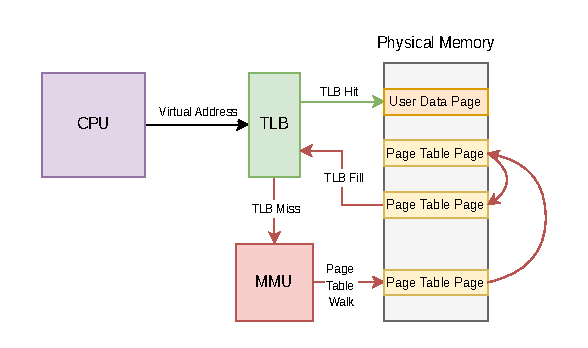
\includegraphics[scale=1.5]{figures/theory_normal_tlb_miss.pdf}
    \caption[Usual TLB Miss]{This figure shows what usually happens when the TLB misses:
        the miss will invoke the hardware state machine page table tree walker; the walker traverses
        the page table tree and if a valid PTE is found, the mapping is added to the TLB. The processor
        then executes the failing instruction again which will then result in a TLB hit}
    \label{fig:theory:normal_tlb_miss}
\end{figure*}
% Virtual Memory using a Mapping Function
\begin{figure*}[ht!]
    \centering
    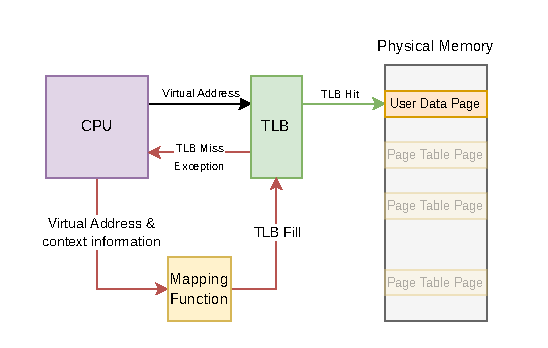
\includegraphics[scale=1.5]{figures/theory_mapping_fx.pdf}
    \caption[Virtual Memory using a mapping function]{Instead of emulating a hardware page table walk in software on
        a TLB Miss exception, a mapping function is invoked that calculates the PTE using arithmetic primitives and tries
        to avoid memory references.}
    \label{fig:theory:mapping_fx}
\end{figure*}

% Kapitel endet mit der Frage was man für die Implementation benötigt?

% -------------------------------------------------------------------------------------------------
%                                            Platform
% -------------------------------------------------------------------------------------------------
% Answers: Welche Platform wird verwendet? Warum?  Was provided die Platform, was nicht?
\section{Platform}
The chosen platform is the xv6 operating system \cite{xv6source}. It is a teaching operating system
used by some MIT courses.\\
xv6 implements the basic Unix Version 6 interfaces, but does so in a very simplified fashion.\\
There is a x86 version and a RISC-V version. For this project, the RISC-V version was chosen.\\
xv6's simplicity and the accompanying handbook \cite{cox2011xv6} make it a good choice for a first
proof of concept.

xv6 will be run on the QEMU \cite{QEMUSource2024} emulator. The QEMU RISC-V emulator implements
all the RISC-V features and extensions that xv6 needs.

Running the operating system on an emulator is a necessity, because the requires the hardware to
throw a TLB Miss exception.\\ The RISC-V ISA does not provide such functionality by default, so
part of the theory and implementation chapters will be dedicated to extending the RISC-V ISA and
the QEMU emulation to support TLB Miss exceptions.
%Implementation Platform
Diese Kapitel betrachtet zwar nur die Theorie des softtlb desings, allerdings muss diese in Kontext
der gewählten Platform gestellt werden und wird daher an manchen Stellen in tieferes Detail der konkreten
Platform eintauchen als man für eine theoretische Ausarbeitung des Designs erwarten würde.
Das ist wichtig um dem späteren Implementierungskapitel den nötigen Kontext zu liefern.\\
Als Platform für die Implementierung wurde der Einfachkeit halber das xv6-riscv educational operating
system \cite{cox2011xv6} gewählt.\\
\textit{Xv6} wird am MIT genutzt um Operating Systems Kurse zu bieten und bietet mit dem Handbuch eine
einfache und verständliche Platform die ein vereinfachtes Unix Version 6 Interface implementiert.\\
Xv6 gibt es in einer x86 version und in einer RISC-V version, es wurde hier die RISC-V version verwendet.
\\
Da im Rahme der Implementierung einer neuen Exception das nutzen echter RISC-V Hardware nicht möglich
ist, muss ein Emulator benutzt werden um die nötigen Änderungen an der ISA zu implementieren und zu nutzen.
Dafür wurde der Qemu Emulator gewählt, da dieser sehr Umfassend und performant ist und außerdem einen
TLB emuliert.
% Zukünftige Idee -> Configurierbarer "stateless" physical frame calculator hw baustein

% Was provided die Platform noch nicht, was muss noch gemacht werden um das Design zu realisieren?
% Implications of programming platform on implementation -> needing to implement TLB Miss
% -------------------------------------------------------------------------------------------------
% -------------------------------------------------------------------------------------------------
%                                            IMPL THEORY
% -------------------------------------------------------------------------------------------------
% -------------------------------------------------------------------------------------------------
% Overview of the different parts necessary to implement the idea
\section{Conceptual Basis for Implementation Modifications}
% What to do to realize this idea? (basically top level overview of the theory and impl chapters)
Dieser Abschnitt enthält die theoretischen Ausarbeitungen zu den einzelnen Bestandteilen die für
die Implementation des Software kontrollierten TLB Miss Handlers benötigt werden. Diese Bestandteile
sind wie folgt:
\begin{itemize}
    \item Die Erweiterung des Qemu Emulators um einen Exceptionwurf bei TLB Miss
    \item Einen Maschine-Mode Traphandler in xv6 der die neue TLB Miss Exception entsprechend behandelt
    \item Eine Möglichkeit um TLB einträge mittels spezieller Instruktionen zu schreiben
\end{itemize}

% -------------------------------------------------------------------------------------------------
%                                            Required Changes
% -------------------------------------------------------------------------------------------------

% What to do to realize this idea? (basically top level overview of the theory and impl chapters)
% New Exception - TLB Miss Exception
% CSRs to write TLBs
% Exception Handler

% Steps necessary to implement Idea -> relating to the implementation

% Architecture: Handle TLB Miss -> Like Liedtke MIPS

% TLB Exception
% TLB Filling



%elaboration on general costs of page table walks -> basically exactly what related
% work motivated their designs with



\todo{elaboration on xv6 here or in fundamentals (or an extra platform chapter)?? -> because theory
    may be independent from the platform in big parts, but still needs to be taken into consideration (like with
    csrs)}



% -------------------------------------------------------------------------------------------------
%                                            TLB MISS EXCEPTION
% -------------------------------------------------------------------------------------------------
% -------------------------------------------------------------------------------------------------
\subsection{TLB Miss Exception}

% -------------------------------------------------------------------------------------------------
\subsubsection{MIPS TLB Exceptions}

% -------------------------------------------------------------------------------------------------
\subsubsection{RISC-V Exceptions}

% -------------------------------------------------------------------------------------------------
\subsubsection{New Exception}


% -------------------------------------------------------------------------------------------------
%                                            Exception Handling
% -------------------------------------------------------------------------------------------------
\todo{ist dieser Abschnitt vielleicht eher der Idee zuzuordnen? So in der Art sollte es
    auf jeden Fall in die Idee, aber vielleicht nicht in diesem Detail, vielleicht nur einmal
    den ''typischen'' controlflow durchgehen und dann einmal den Modifizierten für softtlb}

Damit das Betriebssystem im Falle eines TLB Misses sich um das füllen des TLBs kümmern kann
braucht es zunächst einmal einen Mechanismus um das Betriebssystem wissen zu lassen,
das es zu einem entsprechenden TLB Miss gekommen ist. In Betriebssystemen, die keinen
software managed TLB, wie z.b. MIPS \cite{MIPSArchitectureProgrammers2016} umfassen, ist der
Zugriff auf den TLB in der Regel komplett transparent für das Betriebssystem und somit auch wenn
es zu einem TLB miss kommt. Normalerweiße würde dann die Hardware State Machine aktiviert werden
die dann einen entsprechenden Page Table Walk durchführt um den TLB zu füllen.
\todo{
    explain normal pipeline for TLB misses -> like here + with repeating of fauling instruction
    -> tlb as interface between virtual and physical memory\\
    Aber vielleicht nicht hier
}
Statt das nun aber das MMU anfängt nach dem passenden PTE zu der virtuellen Adresse zu suchen,
soll ein Exception geworfen werden, die das Betriebssystem abfängt um den TLB dann in Software
zu füllen.\\
Im folgenden wird zunächst der allgemeine RISCV-Trap mechanismus betrachtet und dann
wird erleutert wie eine neue Exception in RISC-V hinzugefügt werden kann, bzw. was alles beachtet
werden muss.


% -------------------------------------------------------------------------------------------------
\subsection{Exception Handling}

% -------------------------------------------------------------------------------------------------
\subsubsection{L4/MIPS TLB Exception Handling}

% -------------------------------------------------------------------------------------------------
\subsubsection{Exception Handling in General}

% -------------------------------------------------------------------------------------------------
\subsubsection{xv6 Exception Handler}

% -------------------------------------------------------------------------------------------------
\subsubsection{TLB Miss Exception Handler}
% Compare my implementation to a mips one -> Heiser TLB Fastpath

% Catching New Exception
%   Current xv6 machine mode exception handler ( -> maybe too implementation specific)
%   riscv interrupt mechanism (precice, vectorized)
%   Exception Catching theory, context switch, state save restore
%\section{TLB Miss exception handling}
% Allgemeines über Exception Handling, Context Switches, etc
%\subsection{xv6 exception handling}





% -------------------------------------------------------------------------------------------------
%                                            TLB FILLING
% -------------------------------------------------------------------------------------------------
\subsection{TLB Filling}

% -------------------------------------------------------------------------------------------------
\subsubsection{MIPS TLBs}               % Combine TLB Sections into one ( Multiple TLB designs clash here ...)

%       Starting with MIPS for inspiration on how instructions for TLB manipulation may look like
%       Then continue with a possible RISCV Implementation Idea
%       I-TLB and D-TLB out of scope
% Inspiration: MIPS
MIPS is a good source of inspiration for a possible CSR format design, since it already provides
instructions to modify the TLB.\\
The MIPS64 instruction set manual \cite{MIPSArchitectureProgrammers2016}
shows a number of different instructions concerned with the invalidation, probing, flushing, reading
and writing (indexed and random).\\
The most interesting for a first design would be the \texttt{TLBWR} instruction for writing a TLB
entry at a random index. With a similar instruction in RISC-V, we can already implement a purely
software-controlled virtual memory system.\\
The other types of TLB instructions that MIPS provides are not strictly necesarry,
except for flushing. Without being able to flush existing translations from the TLB,
user mode processes may try to access physical mappings stemming from other processes.\todo{can this even happen? -> why else would we need to flush the tlb??}
But the RISC-V priviledged Architecture already provides this functionality
with the \texttt{sfence.vma} instruction \cite{riscvreader}.

% Replacement policy
%   MIPS -> Indexed writes
A advantage of software-managed TLBs is, that the operating system can implement custom
TLB replacement policies, that may even change depending on workload, programs running
and other circumstances.\\
The default replacement strategy for the MIPS \texttt{tlbwr} instruction is to simply
use the value of the \texttt{C0\_RANDOM} register as the index for the next TLB entry
to be replaced. The name of that register is missleading, because it is not actually a
random value, but it is rather decremented on each instruction\cite{heiserAnatomyHighPerformanceMicrokernel}.\\
It is not clear whether this is a sensible replacement strategy,
but it can be used to ensure that the same TLB slot is not used for every \texttt{tlbwr} if the implementation
does not provide for any further replacement strategy.\\
Some TLB entries can be protecte from this ''random'' replacement by setting a value in the \texttt{C0\_WIRED}
register. The value in this register represents a lower bound, protecting all TLB entries that lie below it.\\
This is useful to keep some mappings in the TLB that are valid all the time.

% TODO should this be here? We should probably have a discussion about xv6 first
%Protected TLB entries in xv6 -> Trampoline page
Having a protected space of TLB entries can especially be useful for global mappings. xv6 employs such a global
mapping for every process and the kernel with the trampoline page.\todo{trampoline page should be explained in fundamentals/platform}

\paragraph{MIPS - TLBWR} The arguments for the instruction need to be written in some
other registers - \texttt{EntryHi}, \texttt{EntryLo0}, \texttt{EntryLo1} and \texttt{PageMask}.


% -------------------------------------------------------------------------------------------------
\subsubsection{RISC-V TLBs}
% Riscv can flush entries of a specific ASID only, this means that it keeps that information
% selective TLB flushing -> RISCV ASIDs (or even no TLB flushing  because VAs contain ASID?)
% Somewhere in the TLB structure
\subsubsection{QEMU TLBs}
% Qemu -> TLB structure, replacement
RISC-V and its extensions currently provide no support for modifying the TLB in software.
RISC-V does however provide a lot of extensibility with the \texttt{Control and Status Registers} (CSRs).\\
CSRs are part of the RISC-V priviledged architecture and are provided by the \texttt{Zicsr} extension\cite{RISCVInstructionSet}.\\

% How is the RISCV Tlb indexed -> Check Qemu source
% -------------------------------------------------------------------------------------------------
\subsubsection{Real TLBs}
% Typical TLB entry format

% -------------------------------------------------------------------------------------------------
\subsubsection{RISC-V CSRs}

% -------------------------------------------------------------------------------------------------
\subsubsection{TLB CSRs}
% Fixed TLB format, but flexibilty of CSR format

% Required Size of CSRs for TLB writing
\begin{figure*}[t]
    \centering
    \begin{bytefield}[bitwidth=\widefigurewidth/39,bitheight=\widthof{~PBMT~}, bitformatting={\tiny\bfseries}, boxformatting={\centering}]{39}
        \bitheader[endianness=big]{38,30,29,21,20,12,11,0} \\
        \bitbox{9}{VPN[2]} &
        \bitbox{9}{VPN[1]} &
        \bitbox{9}{VPN[0]} &
        \bitbox{12}{Page Offset}\\
    \end{bytefield}
    \caption[RISC-V Sv39 Virtual Address]{RISC-V Sv39 Virtual Address}
    \label{fig:theory:sv39va}
\end{figure*}



\todo{TLB CSR Format}

\todo{Hardware dependenc -> still dependent on the TLB structure of RISCV Sv39, VAs and PAs remain, as do PTEs}



% -------------------------------------------------------------------------------------------------
%                                            MAPPING FUNCTION
% -------------------------------------------------------------------------------------------------
\subsection{Mapping Functions}
% -------------------------------------------------------------------------------------------------
\subsubsection{Segmented Mapping}

% Assumptions
%Design of Segmented VM softtlb -> Assumption: Process Memory allocation Model -> Only growing upwards
% Segmentation -> ASIDs -> HW support for Address Space Protection
% -> [jacob1998virtualissues]


% A look at input and output data
% Calculation of addresses

% xv6 Perspective and specifcs (but still theory!) -> Into Impl?
%   Special mappings -> special case in tlb manager (e.g. Trampoline)

% End of Theory: A simple mapping function - TLB Manager
%   TODO What does the reader need to know at this point, e.g. what does need to be decided 
%   in theory to create a TLB Miss Handler design??

% xv6 Process Model
The new memory system needs to be compatible with the existing one. Otherwise the way xv6
user processes are built and structures needs to be changed.\\
The program memory model of xv6 programs is shown in figure \ref{impl:xv6layout}

\begin{figure*}[t!]
    \centering
    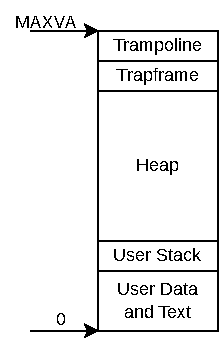
\includegraphics[scale=.5]{figures/prog_vm.pdf}
    \caption[xv6 memory layout]{Virtual memory layout of xv6 processes. Taken from the xv6 book \cite{cox2011xv6}.}
    \label{impl:proclayout}
\end{figure*}

Xv6 processes have their data and text segment and the stack at the very bottom of the virtual
address space \cite{cox2011xv6}.\\
A peak into the implementation of the \texttt{sbrk()} system call also shows us, that the heap
address space grows linearily from low to high addresses.\\
None of the xv6 programs differ from this memory model. There are no pages mapped in the
middle of the address space.\\
The only special cases are the \textit{trampoline} and \textit{trapframe} pages.
\todo{trampoline and trapframe already explained?}

% Segmented memory layout

\begin{figure*}[ht!]
    \centering
    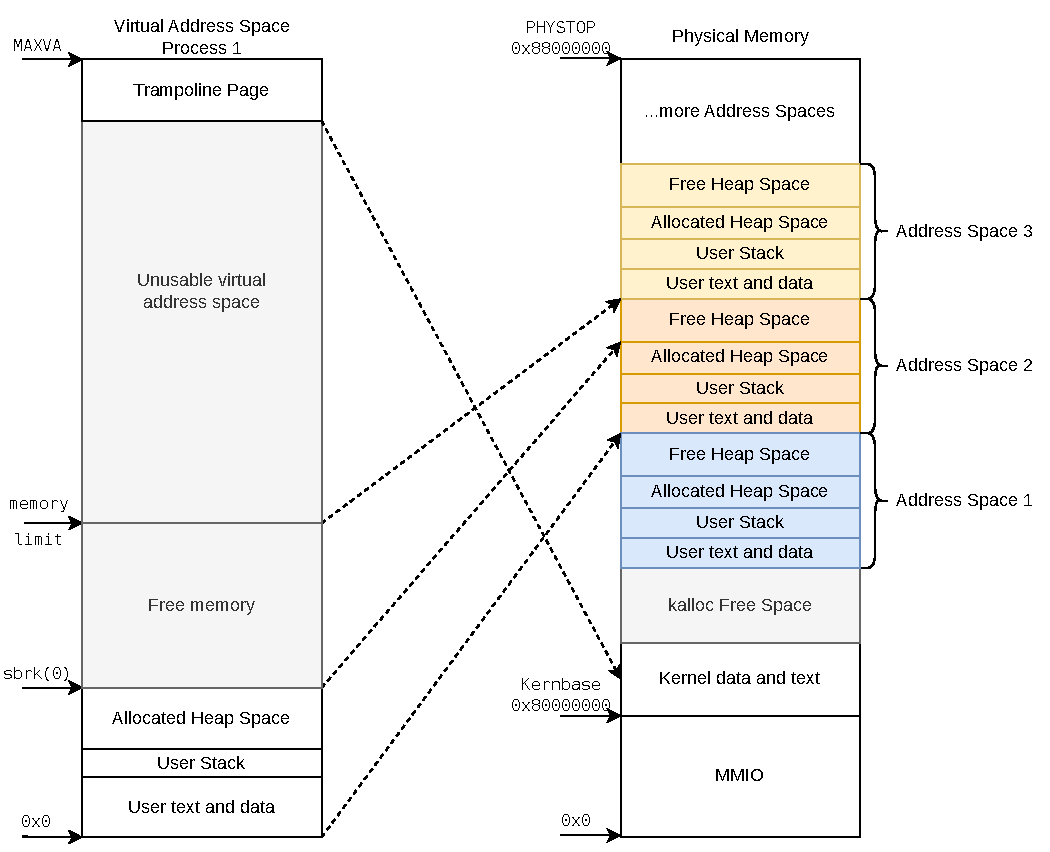
\includegraphics[]{figures/segmented_layout.pdf}
    \caption[Segmented Memory Layout]{\textbf{Segmented Memory Layout}}
    \label{fig:theory:segLayout}
\end{figure*}

\begin{figure*}[ht!]
    \centering
    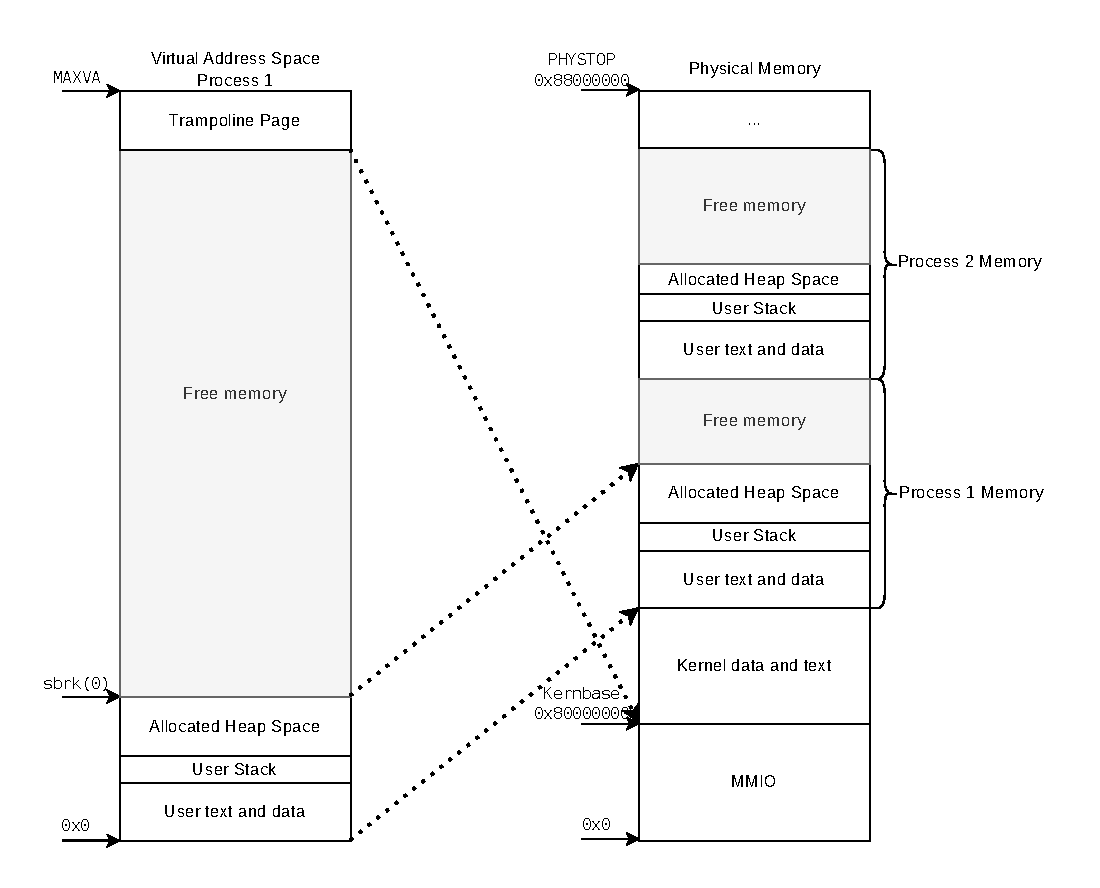
\includegraphics[]{figures/simple_mapping.pdf}

    \caption[Simple Mapping Scheme]{Simple Mapping Scheme}
    \label{fig:theory:simplemapping}
\end{figure*}
% -------------------------------------------------------------------------------------------------
% -------------------------------------------------------------------------------------------------
% -------------------------------------------------------------------------------------------------
% -------------------------------------------------------------------------------------------------

\chapter{Implementation}

\label{chap:impl}

% -------------------------------------------------------------------------------------------------
%                                           General TODOs
% -------------------------------------------------------------------------------------------------


\todo{Add references to documentation at appropiate places}
\todo{ add disclaimer, that most of this information was derived from reading the source code and may in some places not be accurate because the code is pretty complex and
    i have only been at it for a few months}

% TODO viruteller address raum eines xv6 processes
% Qemu implementation TLB vs Echter TLB
% -------------------------------------------------------------------------------------------------
%                                    Chapter structure overview
% -------------------------------------------------------------------------------------------------

%   Source overview
%     QEMU
%     xv6
%   Stage1 - Single Fixed address
%     Qemu - exception
%     xv6 - tlb triggerer
%   Stage2
%     Qemu - TLB CSRs
%     xv6 - Exception Handler, single address tlb fill
%       Exception vector entry -> state save, kernel stack
%   Stage3 - VM PTW with TLB miss handler
%     Qemu -> Extension to all addresses
%     xv6 -> tlb miss handler with ptw
%   Stage4 - Dynamic Segmentation allocation scheme (btw -> link to MIPS?)
%     Qemu -> No more changes needed
%     xv6 -> A lot of changes here
%   Debugging
%   Discussion on implementation
%       Concurrency
%       VM Features
% -------------------------------------------------------------------------------------------------

% High level description of the development steps and their reasoning

% -------------------------------------------------------------------------------------------------
% Section on the rationale for choosing this platform -> or just say that this was chosen and dont rationalize it

% -------------------------------------------------------------------------------------------------
% Introductory section
This chapter summarizes the implementation of the \textit{softtlb} page-table-less virtual memory system. softtlb is a term used secludedly in this paper and refers to the software handling of TLB misses via a exception handler.
The order of the sections in this chapter reflects the implementation process of the softtlb design and a mapping function implemented on top of that design. It consists of the following steps:
\begin{enumerate}
    \item \textbf{TLB miss exception and Exception Triggerer} The first step is about
          the implementation of the TLB miss exception in the QEMU RISC-V emulator. On the xv6-side,
          a user-mode program is added to trigger a TLB miss exception from the shell.
    \item \textbf{Exception Handling and TLB Writing} The second step implements the
          handling of the TLB miss exception by implementing a machine mode exception handler.
          The RISC-V emulation is extended by two new CSRs that facilitate writing TLB from the
          software-side of things.
    \item \textbf{Software Page Table Walk for all Addresses} This step removes the restriction
          in the QEMU emulator to only throw exceptions for a specific address. In the exception handler,
          a page table walk is implemented to now create virtual to physical mappings for all addresses.
    \item \textbf{Segmented Memory Design using software-defined TLB Filling} In this step, the xv6 virtual memory system is completely
          replaced. The new design gets rid of the page table and only uses information present in
          registers to create virtual-to-physical mappings and to fill the tlb.
\end{enumerate}
Each section elaborates on both the xv6 side and the QEMU side of the implementation.
The final section describes debugging techniques that were used or can otherwise be useful for
similar implementations.

\begin{figure*}[t!]
    \centering
    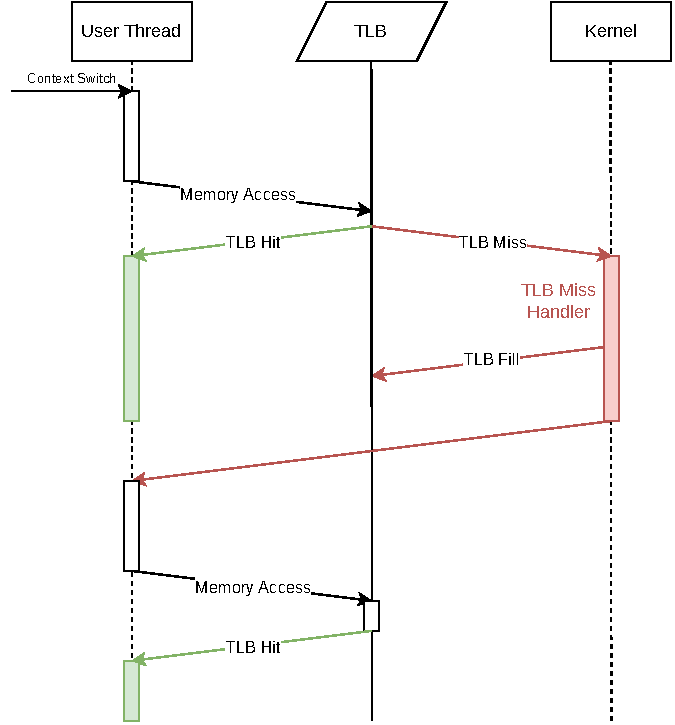
\includegraphics[scale=1]{figures/sequence.pdf}
    \caption[Sequence of actions]{Sequence of action in case of a TLB Hit and Miss}
    \label{impl:sequence}
\end{figure*}


% First step in the development process
% -------------------------------------------------------------------------------------------------
%                                          SECTION STEP 1
% -------------------------------------------------------------------------------------------------
\section{TLB miss exception and Exception Triggerer }
There are two requisites the hardware needs to fulfill in order to do a software-managed TLB fill:
to be a way to signal to the operating system that a TLB miss occurred and there needs to be some
sort of instruction that can be used to write TLB entries.
This step is about the former: Changing the QEMU RISC-V emulator to throw a newly defined \textit{
    TLB miss exception} whenever the TLB misses.
% Why only start with one fixed address?
Changing the whole system to start throwing a TLB miss exception on every virtual address would
make it very hard to debug both first tries at implementing a handler for the exception and the
exception throwing code in QEMU itself.
And not only would the exception be thrown as soon as virtual memory is activated in
\texttt{xv6-riscv:kernel/main.c}, the exception would be thrown
as soon as exceptions are activated and a memory access happens, because QEMU also uses the
\texttt{fill\_tlb} routine to fill the TLB with direct
virtual-to-physical mappings when no virtual memory is used. This speeds up the execution of
the dynamically translated code, as it is able to directly
lookup addresses in the TLB using a fast path \cite{DeepDiveQEMU}.
For this step of the implementation, the QEMU memory system emulation must be changed to throw a
TLB miss exception when a TLB lookup misses. To keep the system running as normal, this will
be done for only one hardcoded address, that is usually not used by xv6.
On the xv6 side, we need a user-level program, that accesses the specific address and thus prompts
the emulated hardware to throw a TLB miss exception.


% -------------------------------------------------------------------------------------------------
\subsection{Address Selection}
The choice for an address to be used for testing the TLB miss exception throwing is easy:
As shown in Figure \ref{impl:xv6layout}, the physical memory map of xv6 has an
area of ``Free memory'' that is managed by the physical memory allocator. The memory allocator
always gives out the next page starting from low to high addresses when a new page is requested
by kernel routines. The address \texttt{0x84fff000} was chosen as a testing address.
Note that the physical memory allocator in \texttt{kalloc.c} will actually touch on to this (or
any address in the range from \texttt{0x80000000} to \texttt{0x88000000}), when initializing
the linked list used to keep track of the free pages \cite{cox2011xv6}.\todo{explain why this
    may be relevant or just leave it out? }
% does not need to be a accessible address now, but later we want to write and read from it

\begin{figure*}[t!]
    \centering
    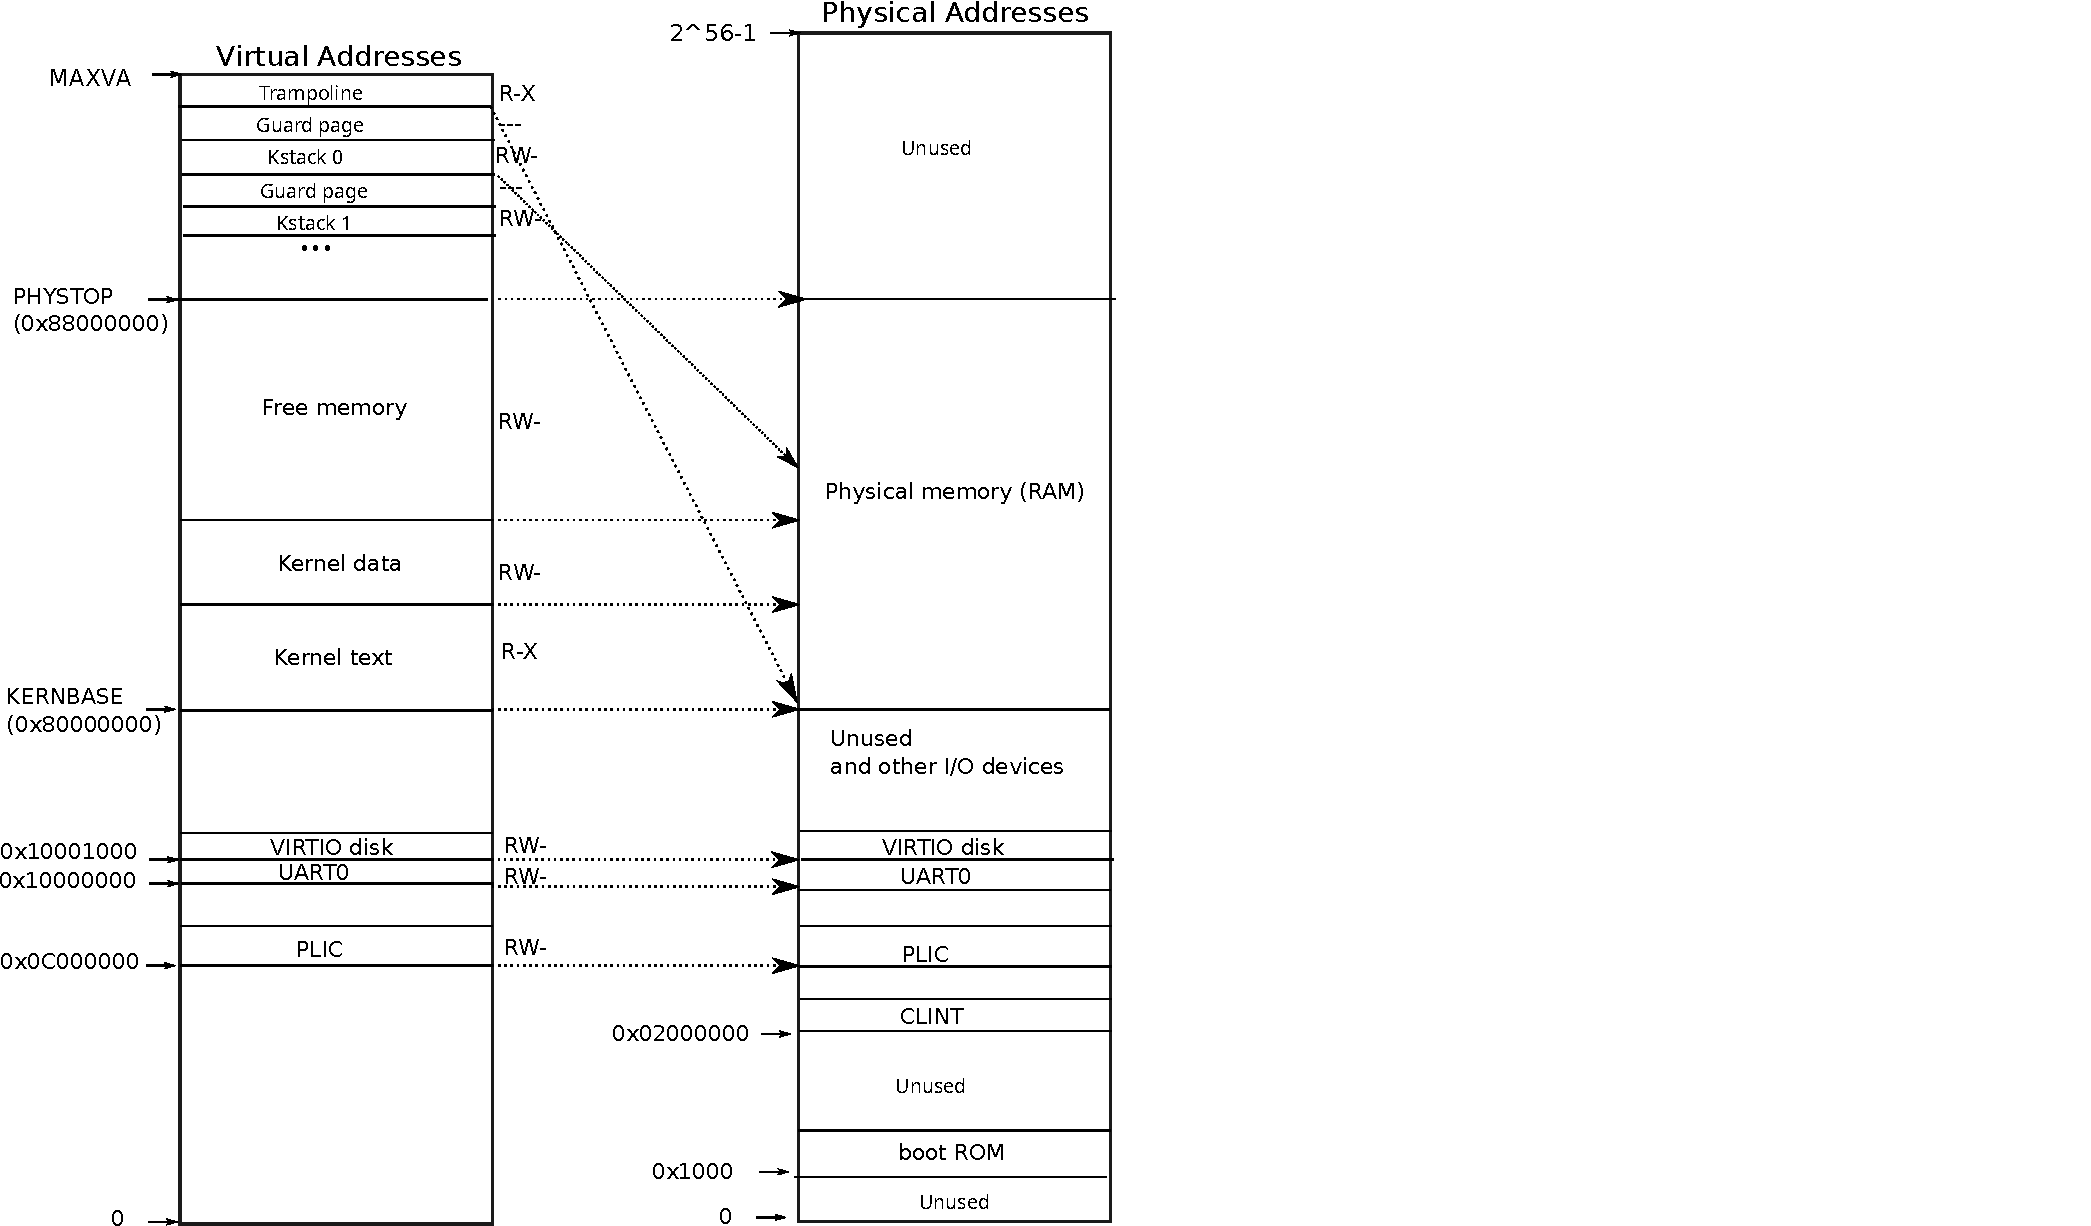
\includegraphics[scale=.5]{figures/xv6_layout.pdf}
    \caption[xv6 memory layout]{The xv6 memory layout and how the kernel virtual address space is mapped on
        the physical address space. Taken from the xv6 book \cite{cox2011xv6}.}
    \label{impl:xv6layout}
\end{figure*}


\subsection{TLB miss exception in QEMU}
%TODO Explain what the riscv_cpu_tlb_fill function does originally - in detail
% TODO discussion and reference to READER/SPECIFICATION on what exception numbers and other constants can be used and are free

% Qemu RISCV  exception adding "tutorial"
%TODO Description of the TLB Exception implementation and how to generally add exceptions to the QEMU plattform
% TODO List of code locations where changes need to be added -> should be usable as back reference for implementing more exceptions

To properly test the implementation, the \texttt{tlb\_fill} function was replaced to throw the
TLB\_MISS exception for
one specified, page-aligned address and to continue normally for every other address.
The implementation is outlined
in Listing \ref{lst:specialCaseTLBfill}.



% riscv_cpu_tlb_switch function
%TODO is this listing really interesting?
\begin{lstlisting}[language=c,float=h!,
    caption={Alternative Implementation for the RISC-V tlb\_fill function with a special case to
    start testing TLB Miss Handler implementations.
    In line 11, a conditional branch is used to only trigger the exception when neither the
    Virtual Memory (as set in the \texttt{satp} \texttt{MODE} field) is bare nor the privilege
    mode is the machine mode.
    If the virtual address is the hardcoded one, a TLB miss exception is thrown, otherwise the
    original functions is called, which will perform a page table walk to find the mapping.},
    label={lst:specialCaseTLBfill}]
bool my_riscv_cpu_tlb_fill(CPUState *cs, vaddr address, int size,
    MMUAccessType access_type, int mmu_idx,
    bool probe, uintptr_t retaddr)
{
    RISCVCPU *cpu = RISCV_CPU(cs);
    CPURISCVState *env = &cpu->env;
    int mode = mmuidx_priv(mmu_idx);
    int vm = get_field(env->satp, SATP64_MODE);
    bool ret = false;

    if(!(vm == VM_1_10_MBARE || mode == PRV_M) &&
            address == (uint64_t)0x84fff000) {
        ret = riscv_cpu_tlb_miss_exception(cs,address,size,access_type, mmu_idx, probe, retaddr);
    } else {
        ret =  riscv_cpu_tlb_fill(cs,address,size,access_type, mmu_idx, probe, retaddr);
    }
    return ret;
}
\end{lstlisting}

% -------------------------------------------------------------------------------------------------


% This section describes the necesarry steps for adding the TLB miss exception to the qemu source
%in comparison with Page fault exceptions
To draw inspiration on how to implement a TLB miss exception in QEMU, you can look at how
page fault exceptions are thrown.
Whenever a page fault exception is triggered, the TLB is checked first to see if there is a mapping
for the input virtual address \cite{QEMUSource2024}. Additionally, RISC-V cores provide the faulting
address of the page fault exception in the \texttt{mtval} register \cite{RISCVInstructionSet}.
The faulting address will also be necessary for handling the TLB miss exception.


% -------------------------------------------------------------------------------------------------

% -------------------------------------------------------------------------------------------------

% Adding new Exception to Qemu RV target
\paragraph{Adding a new exception}to the QEMU emulator requires changes at a number of places. In the following,
the relevant code locations in the QEMU source \cite{QEMUSource2024} are shown.
This may be completely different for other targets, as the exception code is mostly target specific and
this implementation only looked at the RISC-V target.
\begin{itemize}
    \item \texttt{target/riscv/cpu\_bits.h} contains all CPU-definitions specific to the RISC-V target.
          There is also a enum called \texttt{RISCVException} which contains the number-codes for all RISC-V exceptions.
          In choosing a appropiate number for a new exception, one should consult the Privileged Architecture Specification \cite{RISCVInstructionSet}.
          There are specific exception code ranges that are designated for custom use. E.g. the codes 24--32 and 48--63.
    \item \texttt{target/riscv/cpu\_helper.c\:riscv\_cpu\_do\_interrupt\(\)} is the target-specific function
          for triggering interrupts. Here it suffices to add the new exception enum item to the switch case, when
          the new exception is similar in behavior to existing exceptions.
          Here the new exception is simply supposed to jump into an exception handler in the kernel. A lot of exceptions
          like page faults share that behavior.
    \item Finally, if the exception should be delegatable to supervisor mode or user mode, the n-th bit,
          with n being the exception code, needs to be set in the \texttt{DELEGABLE\_EXCPS} definition in \texttt{target/riscv/csr.c}.
          This enables the kernel to delegate the exception to another privilege level by setting the appropriate
          bit in the \texttt{medeleg} and \texttt{sedeleg} CSRs.
\end{itemize}

The code shown in Listing \ref{lst:specialCaseTLBfill} will finally trigger the function shown in
Listing \ref{lst:exceptionThrow}. After executing this function, QEMU will trigger a TLB miss exception as soon
as it gets back to the main execution loop \cite{QEMUSource2024}.

\begin{lstlisting}[language=c,float=h!,
    caption={Setup-Code for raising a TLB Exception. The \texttt{cs-\textgreater exception\_index} variable needs
    to be set to the custom \texttt{TLB Exception} enum value. The \texttt{env-\textgreater badaddr} variable
    will end up in the \texttt{mtval} register. The address will be page-aligned first, by zeroing out the
    lowest 12 bits. This is used to encode the \texttt{mmu\_idx} into the faulting address. Why this is
    necessary is explained in Section \ref{sect:tlbwrite}},
    label={lst:exceptionThrow}]

    static void raise_tlb_exception(CPURISCVState *env, target_ulong address,
                                MMUAccessType access_type,
                                /*unnecessary?*/ bool pmp_violation,
                                bool first_stage, bool two_stage,
                                bool two_stage_indirect, uint8_t mmu_idx) {
        CPUState *cs = env_cpu(env);

        cs->exception_index = RISCV_EXCP_TLB_MISS;
        env->badaddr = ( address & ~( (1 << 12) - 1)) | mmu_idx;
        env->two_stage_lookup = two_stage;
        env->two_stage_indirect_lookup = two_stage_indirect;
    }

\end{lstlisting}

% -------------------------------------------------------------------------------------------------


\subsection{Exception Triggerer}
% TODO TLB exception trigger
To properly test the changes introduced to the QEMU emulator, there needs to be some way to
trigger a TLB exception.
By implementing this as a user-level program, the exception can be triggered using the xv6 shell.

\textbf{Adding a new user-level Program to xv6} only needs you to add a new \texttt{.c} file to the user subfolder
and to add the name of the generated binary ( name of \texttt{.c} file prefixed with a \texttt{\_})
to the list of user binaries in the makefile.
The new \texttt{.c} file only needs a \texttt{main} function and should also include the \texttt{user.h}
file to gain access to some preimplemented function and system call wrappers \cite{xv6source}.

The final exception triggerer may look something like this:

\begin{lstlisting}[language=c,float=h!,label{impl:excptTrigger},caption={\textbf{Exception Triggerer} Trying to
    load from a hardcoded address prompts the emulated hardware to trigger a TLB miss exception.}]
    #include "kernel/types.h"
    #include "user/user.h"

    void do_tlb_exc(void) {
        __asm__("li s2, 0x84fff000\n\t \
                lw s4, 0(s2)\n\t");
        register int *foo asm ("s4");
        printf("%x\n", foo);
        return;
    }

    int main(int argc, char *argv[]) {
        do_tlb_exc();
        //exit(0);
    }
\end{lstlisting}



The program first loads the hardcoded address into a register and then tries to load a word from this address.
If the implementation of the \texttt{TLB miss exception} was done correctly, the process will trap to the kernel
and the kernel will print out an error message, as it does for all exceptions that either have unknown exception
numbers or do not have a exception handler implemented \cite{cox2011xv6}.
If the exception was not properly implemented, the kernel would report a load page fault exception.

\todo{add xv6 shell output at this stage progression - should be a error printed by the kernel exception handler}
% -------------------------------------------------------------------------------------------------
%                                       END OF SECTION - STEP 1
% -------------------------------------------------------------------------------------------------



% Second step: Extending the tlb miss handling to be used for all addresses -> implementing a softvm ptw
% -------------------------------------------------------------------------------------------------
%                                         SECTION - STEP 2
% -------------------------------------------------------------------------------------------------
\section{Exception Handling and TLB Writing}
\label{sect:tlbwrite}

Now that the new \textit{TLB miss exception} can be triggered by a user-level program, there needs
to be an exception handler in the kernel that will create virtual-physical mappings and add them to the
TLB.
This section will first go into a general description to add new CSRs to the RISC-V QEMU emulation and
will then elaborate on the specific implementation for the TLB CSRs.
The section ends with the implementation of the exception handler.

% TODO Why does the mmuidx need to be encoded into the faulting address -> Explain


% -------------------------------------------------------------------------------------------------
\subsection{Adding CSRs to RISC-V/QEMU}

% Relevant Code locations
Following code locations are relevant for CSRs in the RISC-V/QEMU emulation source code \cite{QEMUSource2024}:
\begin{itemize}
    \item \texttt{disas/riscv.c} Contains a big switch case with all the CSR number to CSR name mappings.
          Name and number of new CSRs need to be added there.
    \item \texttt{target/riscv/cpu\_bits.h} contains definitions for all CSR numbers.
          While it is not strictly necessary to add another definition for new CSRs here, readability and maintainability
          of the code increases if a more descriptive definition name is used instead of a magic constant.
    \item \texttt{target/riscv/cpu\_cfg.h} contains a structure called \texttt{RISCVCPUConfig}. Every emulated RISC-V hart
          has this structure to expose all the extensions that the hart supports. \todo{hart already known?}
          The structure has a boolean flag for every extension that is currently supported by the emulator.
          New extensions should get their own flag in this struct.
          Similar entries also need to be added to the \texttt{isa\_edata\_arr} and \texttt{riscv\_cpu\_extensions} arrays in \texttt{target/riscv/cpu.c}.
    \item \texttt{target/riscv/csr.c} contains the implementation for all CSRs. The \texttt{riscv\_csr\_operations csr\_ops[]}
          array is essential for adding callback functions to CSR numbers.
          For every new CSR, a struct of the type \texttt{riscv\_csr\_operations} must be added to that array using the
          CSR number as an index. This struct is comprised of multiple function pointers, which deal with
          \begin{itemize}
              \item Checking if the hart implements the CSR
              \item Reading from the CSR
              \item Writing to the CSR
              \item Combined read/write
              \item 128 bit read/writes
          \end{itemize}
\end{itemize}
%Implementation of CSRs

As previously mentioned, the CSRs have some index ranges for new, custom CSRs. For the implementation
of TLB write CSRs, the indexes \texttt{0xBEE} and \texttt{BFF} have been selected.
Using these constants and the steps above, two new instructions\todo{are these actually instructions} can be realized.

\subsection{CSR Callback Implementation} Apart from the above-mentioned steps to add new CSRs to the emulator, the
main logic of the implementation is in the callbacks referenced in \texttt{target/riscv/csr.c}.
The implementation of these callbacks is strongly dependent on the structure of the data that is written to
the CSRs. Fundamentally, these callbacks act as a bridge between the exposed ISA and the implementation of
that instruction set in software.
As previously mentioned, two new CSRs will be needed to implement the TLB-writing. \todo{ PUT THIS IN THE THEORY PART about CSR format and number: In theory, it would
    also be possible to implement the functionality using only one CSR, by just taking the faulting address from the mtval register, but
    this paper focuses on the proof of concept of the design and not on the optimization }
The implementations
of the write-callbacks look as follows:


% Callbacks

\begin{lstlisting}[language=c,float=h!,
    label={lst:tlbh}]
    static RISCVException write_tlbh(CPURISCVState *env, int csrno, target_ulong new_val)
    {
        env->tlbh = new_val;
        return RISCV_EXCP_NONE;
    }
\end{lstlisting}
The implementation of the \texttt{tlbh} CSR write, does not do anything else but saving the value
that is written to it to the environment of the CPU.
This is because the theory specifies\todo{is it specified yet?}, that the TLB entry will only
be written to the TLB when the write to the \texttt{tlbl} CSR has succeeded.

\begin{lstlisting}[language=c,float=h!,
    label={lst:tlbl}]
    static RISCVException write_tlbl(CPURISCVState *env, int csrno, target_ulong pte)
    {

        target_ulong tlb_size = TARGET_PAGE_SIZE;

        CPUState *cpu = env_cpu(env);
        vaddr addr = env->tlbh;
        hwaddr paddr = ((pte & ~(PTE_RESERVED)) >> 10) << 12;

        int mmu_idx = addr & (tlb_size - 1);

        int prot = pte & (PTE_R | PTE_W | PTE_X | PTE_V );

        addr &= ~(tlb_size - 1);
        paddr &= ~(tlb_size - 1);

        tlb_set_page(cpu, addr, paddr, prot, mmu_idx, tlb_size, false);

        env->tlbh = 0;
        env->tlbl = 0;

        return RISCV_EXCP_NONE;
    }
\end{lstlisting}
\todo{all these code lines need a theoretical foundation in the fundamentals chapter (BTW, the format
    still adheres to PTEs!)}
The value written to the \texttt{tlbl} CSR adheres to the same format as the RISC-V Sv39 PTEs (As shown in section \ref{fund:sv39}).

To get the page-aligned physical address and to get rid of the access bits stored in the lower 10 bits,
the value will first be right shifted by ten and then left shifted by 12 bits.
The topmost bits are specified to be all zero, as explained in the fundamentals chapter \cite{RISCVInstructionSet}.

In line 10, the \texttt{mmu\_idx} is extracted from the lowest 11 bits of the virtual address. This is
necessary, because QEMU uses up to 16 different MMU modes with dedicated TLBs \cite{QEMUSource2024}.
Whenever QEMU performs a TLB lookup, it does so in a specific MMU mode. This MMU mode is clear when
a TLB entry is retrieved, it is however not clear when a TLB entry is written.
To still fill the correct TLB, the \texttt{mmu\_idx} is transferred to the exception handler as part
of the faulting address in \texttt{mtval} and then back to the emulator via the TLB write CSRs.

The following lines deal with extracting the protection bits from the PTE and with page-aligning
the virtual and physical addresses. Finally, a preexisting QEMU function is invoked to add
a new entry to the emulated TLB and the CSR values are cleared.
The return value \texttt{RISCV\_EXCP\_NONE} indicates that nothing out of the ordinary happened.

This is all that needs to be done to add CSRs for TLB filling to the QEMU RISC-V emulator.


\todo{discussion of implementation at the end of this chapter: shortcommings, comparison QEMU - MIPS, comparison xv6 new vm - other vm -> eval??}

% -------------------------------------------------------------------------------------------------

\subsection{TLB miss exception Handler}
% Previous state of xv6 machine mode trap handler
%   -> Only for Timer Interrupt
%   -> Small amount of saved registers
% TODO TLB fill manager
% Changes -> Vectored mode to keep timer interrupt as is, just need to move it
With capabilities to write TLB entries in place, an effective exception handler can be implemented.

\paragraph{xv6 Machine-Mode Trap Handler} The xv6 machine-mode trap handler only deals
with the timer interrupt. All other interrupts and exceptions are delegated to the supervisor
mode. This allows the trap handler to be very small and very specific to the timer interrupt \cite{cox2011xv6}.
It thus only needs to store two registers to memory to make enough room in the register file
to reset the timer and invoke the scheduler.
Adding another trap to be handled adds more complexity, as the trap number needs to be checked
and the code needs to branch to the right routines.

But it can also be completely avoided to touch the timer code at all. xv6 uses trap vectoring
mechanism in \textit{direct} mode. In direct mode, all traps jump to the same address.
Using the \textit{vectored} mode makes all \textit{exceptions} jump to the address set
in the \texttt{mtvec BASE} field but all \textit{interrupts} are set the program counter
to \texttt{BASE} plus four times the interrupt cause \cite{RISCVInstructionSet}.

So to add machine mode exception handlers with disrupting the existing code as little as possible only
requires changing the trap vectoring mode to \texttt{vectored} mode and moving the timer interrupt code
to the correct offset.

\begin{lstlisting}[language=diff]
-    w_mtvec((uint64)timervec);
+    w_mtvec((uint64)mtvec_vector_table | 0x1);
\end{lstlisting}

The changes for changing the mode are trivial. Only the one bit indicating the \texttt{vectored} mode
needs to be set.
Placing the timer vector at the correct offset from the default trap handler vector can be achieved by
filling the space between the base address and the timer vector with no-operations. The same could be
achieved with linker directives.
The interrupt number for the timer interrupt is \texttt{0x7}, this puts the timer interrupt vector
at a positive \texttt{0x1c} offset from the base address.

\begin{lstlisting}[language={[RISC-V]Assembler},float=h!,
    label={lst:defaultTrapHandler}, caption={Vectored Trap Handler Routine}]
mtvec_vector_table:
IRQ_0:
        j default_exception_handler
        nop
IRQ_1:
        j default_vector_handler
        nop
IRQ_2:
        j default_vector_handler
        nop
IRQ_3:
        j default_vector_handler
        nop
IRQ_4:
        j default_vector_handler
        nop
IRQ_5:
        j default_vector_handler
        nop
IRQ_6:
        j default_vector_handler
        nop
IRQ_7:  # timer handler
        j timervec
\end{lstlisting}

% TODO verifying the placement of addresses and symbols using the name utility

RISC-V provides 4 bytes for every interrupt request (IRQ) and the default trap handler. This is not enough
to implement proper trap handling, so these 4 bytes are typically spent jumping to a more elaborate trap
handling routine.

Now any machine-mode exception (that is not delegated to a lower-privilege mode) sets the program counter
to the address of the \texttt{mtvec\_vector\_table} label. The next jump brings the execution into
the default exception handler.
The timer interrupt will jump directly to the \texttt{IRQ\_7} label.

\paragraph{Store/Load Sandwich} The idea behind the \textit{softtlb} design is to not use as many of the five
memory references modern architectures need for a page table walk \cite{intel5LevelPaging5Level2017}. But
for a first proof of concept, it is helpful to not have to think about which registers to use and to not optimize
away all unnecessary memory references before the design even works.
That is why the first thing the default exception handler will do is to store the current state of the register
file.
This is essential so that, once returned to the context that triggered the TLB miss, execution can continue
as if nothing happened.
After storing the state and running the exception handler, the state must again be loaded into the registers.

\todo{use minipages to have text and listing side by side ? https://latex.org/forum/viewtopic.php?t=6652}
\begin{lstlisting}[language={[RISC-V]Assembler},float=h!,
    label={lst:defaultTrapHandler}, caption={Store/Load Sandwich}]
default_exception_handler:

    csrrw a0, mscratch, a0
    sd sp, 40(a0)

    ld sp, 48(a0)
    csrrw a0, mscratch, a0

    # make room to save registers.
    addi sp, sp, -256

    # save the registers to the hart stack
    sd ra, 0(sp)
    sd gp, 16(sp)
    ...
    sd t5, 232(sp)
    sd t6, 240(sp)

    addi s0, sp, 256 # Set Frame Pointer

    # ??
    # csrr t0, sscratch
    # sd t0, 8(sp)

    # TODO Pass args to fx

    # csrr a0, mtval
    # csrr a1, satp

    call machine_default_exception_handler


    # restore registers from hart stack
    ld ra, 0(sp)
    ld gp, 16(sp)
    ...
    ld t5, 232(sp)
    ld t6, 240(sp)

    addi sp, sp, 256

    csrrw a0, mscratch, a0

    sd sp, 48(a0)
    ld sp, 40(a0)

    csrrw a0, mscratch, a0
    mret

\end{lstlisting}
\todo{side by side}
Most of the load/stores have been omitted to not flood the listing.
In between the store and load blocks, the \texttt{machine\_default\_exception\_handler} C function is called. This is
where the implementation differentiates between the different exception numbers and calls exception handlers
specific to the exceptions.
In xv6, all other exceptions but the new TLB miss exception are handled in supervisor mode, so there are
no handlers for other exceptions.

\begin{lstlisting}[language={C},float=h!,
    label={lst:defaultTrapHandler}, caption={Exception Switch-Case Statement}]
    void machine_default_exception_handler() {
        switch (r_mcause()) {
            case NONE:
            case INST_ADDR_MIS:
            case INST_ACCESS_FAULT:
            case ILLEGAL_INST:
            case BREAKPOINT:
            case LOAD_ADDR_MIS:
            case LOAD_ACCESS_FAULT:
            case STORE_AMO_ADDR_MIS:
            case STORE_AMO_ACCESS_FAULT:
            case U_ECALL:
            case S_ECALL:
            case INST_PAGE_FAULT:
            case LOAD_PAGE_FAULT:
            case STORE_PAGE_FAULT:
            default:
                unhandled_exc(r_mcause(), r_mtval());
                break;
            case TLB_MISS:
                tlb_handle_miss(r_mtval(), r_satp());
                break;
        }
    }
\end{lstlisting}

Finally, the \texttt{tlb\_handle\_miss()} functions is called with the faulting address and the \texttt{satp} register
value as arguments.
The initial implementation simply calls the new \texttt{tlbh} and \texttt{tlbl} CSR instructions with and then
returns.
% Description of tlb handler and call of tlbh and tlbl
\begin{lstlisting}[language={C},float=h!,
    label={lst:defaultTrapHandler}, caption={Simple TLB miss exception handler for a single fixed address}]
void tlb_handle_miss(uint64 addr, uint64 usatp) {
  //uint64 *paddr = kalloc();
  w_tlbh(addr);
  w_tlbl((uint64)addr+(uint64)0x1000);
  return;
}
\end{lstlisting}

Note that this implementation does not yet use the format for the \texttt{tlbh} and \texttt{tlbl} CSRs specified
in the theory section \ref{chap:theory}.
Merely the faulting address and the intended mapping are written to the registers.

% HERE TODO explain the implication for implementation
\subsection{Testing}
Listing \ref{lst:defaultTrapHandler} already shows a part of the setup to test that the mapping actually worked.
When the mapping worked, it should be possible to read a value from the mapped page.
The user-level exception triggerer already tries to do just that.
With the mapping working, the output of the program looks as follows:

\todo{add console output}

The value \texttt{0xDEADBEEF} that was read from the mapped page is not a coincidence:
For testing purposes, the page \texttt{0x85000000} was filled with \texttt{0xDEADBEEF} bit patterns.

The address for the physical ''testing'' page was deliberately chosen to be \texttt{0x85000000} and not
\texttt{0x84fff000} (like all the hardcoded testing addresses) to make sure that there is no accidental physical
mapping happening.


\todo{add xv6 shell output at this stage progression - no more exception printing, xv6 should read deadbeef now}

% -------------------------------------------------------------------------------------------------
%                                       END OF SECTION - STEP 2
% -------------------------------------------------------------------------------------------------



% -------------------------------------------------------------------------------------------------
%                                       STEP 3 - New VM
% -------------------------------------------------------------------------------------------------
\section{Software Page Table Walk for all Addresses}
After implementation step 2, we now have a modified QEMU RISC-V emulator, which will throw the new
TLB miss exception when the TLB misses.
We have also extended the xv6 operating system to catch said exception and to create a virtual-physical
mapping for the faulting address.
The mapping is created by writing new TLB entries using newly implemented TLB CSRs.

Currently, all of this only works for one specific ''testing'' address. This step now elaborates on
how the scheme is extended to be used for all addresses.
To not change too much at once, the page table walk that would typically be done in hardware is
implemented as part of the TLB miss exception handler.

\subsection{TLB miss exception for all Addresses}
The changes introduced to QEMU are simple: Essentially, only the condition checking if the given address is
the ''testing'' address needs to be changed.
The final implementation looks as follows:

\begin{lstlisting}[language=c,float=h!,
    caption={},
    label={lst:updatedTLBFill}]
    bool my_riscv_cpu_tlb_fill(CPUState *cs, vaddr address, int size,
                        MMUAccessType access_type, int mmu_idx,
                        bool probe, uintptr_t retaddr)
    {
        RISCVCPU *cpu = RISCV_CPU(cs);
        CPURISCVState *env = &cpu->env;
        int mode = mmuidx_priv(mmu_idx);
        int vm = get_field(env->satp, SATP64_MODE);

        //No address translation in m-mode
        if(vm == VM_1_10_MBARE || mode == PRV_M) {
            int tlb_size = 4096; //TODO Get from PMP?
            hwaddr pa = address;
            int prot = PAGE_READ | PAGE_WRITE | PAGE_EXEC;
            tlb_set_page(cs, address & ~(tlb_size - 1), pa & ~(tlb_size - 1),
                        prot, mmu_idx, tlb_size, true);
            return true;
        }
        riscv_cpu_tlb_miss_exception(cs,address,size,access_type, mmu_idx, probe, retaddr);
        return true;
    }
\end{lstlisting}

Note that in comparison to the previous implementation (as shown in figure \ref{lst:specialCaseTLBfill}), the
call to the original \texttt{riscv\_cpu\_tlb\_fill} function is not called anymore.
Either a TLB miss exception is raised, or the TLB is filled with an identity mapping if either the current
privilege mode is the machine mode or the virtual memory system is configured to use identity mappings only
\cite{RISCVInstructionSet}.

% -------------------------------------------------------------------------------------------------

\subsection{Software Page Table Walk}


\begin{figure*}[ht!]
    \centering
    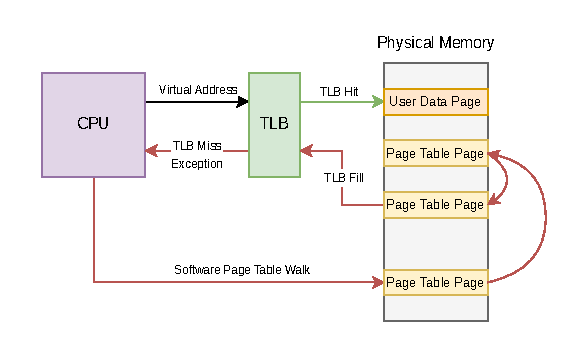
\includegraphics[scale=1.5]{figures/theory_sw_ptw.pdf}
    \caption[Software Page Table Walker]{Instead of transfering control over to the MMU to fill in the missing mapping,
        the TLB miss exception invokes a software page table walker}
    \label{fig:theory:sw_ptw}
\end{figure*}

Now that the TLB miss exception is thrown for every faulting address, it also needs to be handled
for every address.
Even though the goal is to explore alternatives to virtual memory using page tables, we will
use a software implementation of the hardware page table walk. This is to verify that the
general setup including exception invocation, exception handling and TLB writing works as
expected.
Listing \ref{lst:softptw} shows the implementation.

\todo{The listing seems to be way broader than it needs to be}
\begin{lstlisting}[language=c,float=t,
    caption={\textbf{TLB miss exception Handler with Page Table Walk}
    The \texttt{walk\_pt()} function walks the Sv39 page table with the base address
    encoded in the \texttt{satp} register. If a PTE with the valid bit set is found, the function
    returns the address encoded in the PTE.
    Otherwise, the function returns \texttt{0}.},
    label={lst:softptw}]
#define SATP2PA(satp) ((satp << 12) & ~(0xffull << 44))

pte_t *
walk_pt(uint64 satp, uint64 va)
{
  uint64 *pt = (uint64*)SATP2PA(satp);
  if(va >= MAXVA)
    panic("walk");
  for(int level = 2; level > 0; level--) {
    pte_t *pte = &pt[PX(level, va)];
    if(*pte & PTE_V) {
      pt = (uint64*)PTE2PA(*pte);
    } else {
      return 0;
    }
  }
  return &pt[PX(0, va)];
}

void tlb_handle_miss(uint64 addr, uint64 satp) {
    w_tp(r_mhartid());
    pte_t *pte = walk_pt(satp, addr);
    w_tlbh(addr);
    uint16 prot =  PTE_R | PTE_W | PTE_U | PTE_V;
    w_tlbl(*pte | prot);
    return;
}
\end{lstlisting}

\todo{To make it easier to understand -> Architectural overview of the memory path after each implementation step?}

If the \texttt{walk\_pt()} function returns 0, the virtual address lead to no valid PTE. This is a
page fault and would raise a page fault fitting the faulting instructions type of access \cite{tanenbaumOS}.
As xv6 does not handle page faults other than by killing the program \cite{cox2011xv6} this
paper will not go into more detail of raising and triggering page faults for the \texttt{softtlb}
design.


% -------------------------------------------------------------------------------------------------
%                                               STEP 4
% -------------------------------------------------------------------------------------------------

\section{Segmented Memory Design using software-defined TLB Filling}

After step 3, xv6's virtual memory system runs completely without using the (emulated) page table
walking state machine:
Instead of invoking the page table walker, a TLB miss triggers a exception. This exception is handled by the
operating system kernel and a TLB entry for the faulting address is generated.
Yet at this point, we have not really won anything. We only moved the page table walking to the software side,
which would certainly be slower at traversing the page table than a real MMU \cite{jacob1998look}. And that
even if we ignore the expensive context switch that needs to be performed when the exception handler is invoked.

While we did not gain any performance, there is now the opportunity to modify the virtual memory system
completely in software. We do not need to adhere to the rigid structures \cite{tanenbaumOS} of the memory management hardware anymore.
We gained a great deal of flexibility.

The rest of this section explores a first idea of how a table-based virtual memory system can be
replaced by essentially a simple function that does not require expensive memory accesses.

The initial idea, as presented in the theory chapter, is a segmented memory design. It splits the total
available memory into parts of equal size, also called segments.
Each new process acquires one of those segments, if there are any left. If none are left, process creation fails.

\todo{basic assumption to make this work: xv6 process memory model -> should be mentioned here and explained in detail in theory}
% TODO Concept of AS used here -> distinct from hard ware mechanism, but could be used for it
\subsection{Address Spaces}
As with segmentation, the available physical memory is split into evenly sized portions\todo{is it? Cite!}
from now called address space. When a new process is started it tries to acquire an address space by
checking whether there is a free one and then claiming that free address space.
The number of address spaces will thus limit the number of concurrently running programs.

To keep track of which process acquired which address space, the kernel keeps an integer array of process IDs.
This array has a size equal to the number of address spaces (NAS).
For a newly created process to acquire an address space, the kernel will (synchronized by a spinlock \cite{cox2011xv6})
iterate through the array to find a array slot with the value 0. It then writes the process ID into that array.
The process creation fails if there are no more array slots set to 0.
The address space ID (ASID) acquired by the process is also written to the processes control block (PCB).

NAS is set via a preprocessor definition and thus set at compilation time. More elaborate implementations
could also allow dynamic resizing of address spaces to provide space for more processors.\todo{configuration
    towards ones needs -> embedded systems may need a fixed number of processes, or have a maximum amount}

Using the ASID, the address range for a process can be calculated very easily. The macros in listing \ref{lst:macros}
are used in different parts of the code to calculate different addresses related to an Address Space.

\begin{lstlisting}[language=c,float=h!,
    label={lst:macros}]
    #define MAX_AS_MEM ((((PHYSTOP - (PGROUNDUP((uint64)end))) / (NAS + 1)) >> 12 )<< 12)
    #define AS_START(asid) (PGROUNDUP((uint64)end) + ((asid) * MAX_AS_MEM))
    #define AS_N(index, asid) (PROC_START(asid) + (index * (0x1000)))
    #define AS_END(asid) ((PGROUNDUP((uint64)end) + ((asid + 1) * MAX_AS_MEM))-0x1000)
\end{lstlisting}

\subsection{Mapping function for Segmented Memory}
The ASID of a process is the foundation for calculating the virtual to physical mapping in the exception handler.
The only other information required is the faulting address.
\todo{theory needs to explain that the asid is transfered via SATP reg}

The ASID can be used to calculate the actual physical address at which the Address Space starts.
The faulting address, which would, according to the xv6 process memory model, be an address in the low
end of the virtual memory space, will provide the offset into the Address Space.

Listing \ref{lst:handler} shows the implementation for the TLB miss exception handler.

\begin{lstlisting}[language=c,float=h!,
    label={lst:handler}]
#include "defs.h"
#include "param.h"
#include "types.h"
#include "riscv.h"
#include "memlayout.h"

#define SATP2ASID(satp) ((satp << 4) >> 48)

extern char trampoline[];
paddr get_mapping(vaddr addr, uint16 asid) {

  //special case for trampoline, which is in every address space at the same address
  // (except for the physical one!)
  if(PGROUNDDOWN(addr) == TRAMPOLINE) {
    return (uint64)trampoline;
  }
  if(asid == 0) {
    //Kernel -> direkt mapping
    //TODO special mappings
    return addr;
  } else {
    //mappings for processes
    //TODO trapframe and trampoline mappings
    if(PGROUNDDOWN(addr) == TRAPFRAME) {
      return TRAPFRAME_FROM_ASID(asid);
    }

    //Base case
    uint64 vpage = PGROUNDDOWN(addr);
    if(vpage >= MAX_AS_MEM - (0x1000 * 4)) {
      //Error, address out of range
      panic("tlb_manager: address to high!");
    }
    return AS_START(asid) + vpage;
  }
  return 0;
}

void tlb_handle_miss(vaddr addr, uint64 satp) {
  w_tp(r_mhartid()); //fix problems with locks based on cpuid()

  //TODO Locks!
  //TODO buffering printer, only prints completed lines
  //uint16 mmuid = addr & 0xfff;
  vaddr addr_no_mmuid = addr & ~0xfff;
  //printf("tlb_manager: addr=%p satp=%p mmuid=%d\n", addr_no_mmuid, satp, mmuid);
  paddr pa = get_mapping(addr_no_mmuid, SATP2ASID(satp));

  w_tlbh(addr);
  //TODO all access rights for now
  uint16 prot =  PTE_R | PTE_W | PTE_X | PTE_V | ((SATP2ASID(satp) != 0) ? PTE_U : 0);
  w_tlbl(PA2PTE(pa) | prot);
  return;
}
\end{lstlisting}

\todo{check tex comments here}
% TODO it is not enough to simply change the tlb miss manager, because other
%   parts of te OS still use the VM system for stuff
%       What are these parts that interact with the os?
%       How can be made it fit this scheme?

\subsection{Special Mappings}
xv6 needs a trampoline page mapped into the address space of the process for system calls to work properly (see chapter \ref{chap:theory}).
In both the kernel and in the user processes, it is mapped to the highest possible, virtual page.
If a address on this page is encountered, the handler will map it to the physical address of the trampoline page.
The handler takes the same approach for the \texttt{TRAPFRAME} page set just below the trampoline.

\subsection{Further Changes to the OS}
Other than the exception handler, other parts of the OS need to be changed to fit the new memory management scheme.

\paragraph{Physical Memory Allocator} % Rewrite below version in new context
Demand paging of the virtual memory system was the main customer of the physical memory allocator.
But some modules like the virtio disk and pipes also rely on being able to access physical pages. Thus, it is not
possible to get rid of the physical allocator completely.
Here, its managed memory is merely reduced by assigning it the memory area of the Address Space with index 0.

\paragraph{\texttt{copyin() copyout()}} The copyin() and copyout() functions are used to copy data between
user space and kernel. They traverse the page table tree to acquire the physical location for the data
to be either copied in or copied out.
Both of those function rely on the \texttt{walkaddr()} function to do the walking for them.
The implementation can be changed to call the \texttt{tlb\_manager.c:walk\_addr()} function instead.

\paragraph{Process Loading} % No page table creation, asid allocation, also no destruction, % Parsing elf directly into AS
\todo{write}
\paragraph{sbrk()}The \texttt{sbrk()} system call is used by the program to increase the size
of the programs data segment. Typically, this call would demand a new page from the physical memory allocator
and then add a new PTE to the page table.
This system call normally returns the previous program break if it was successful (so basically a pointer to
the new program area) and \texttt{-1} if it was not successful.
Instead, this design checks if the program size would increase to be bigger than the maximum program size and
then return \texttt{-1} if it is and the previous program break otherwise.


% -------------------------------------------------------------------------------------------------
%                                    END OF SECTION - Step 4
% -------------------------------------------------------------------------------------------------



% TODO Should this be an appendix?
% -------------------------------------------------------------------------------------------------
%                                         SECTION - Debugging
% -------------------------------------------------------------------------------------------------
\section{Debugging}
When making simultaneous changes to both the Qemu emulator and xv6, it can be difficult to determine where bugs originate from. This section first describes how to debug Qemu and xv6 individually and then outlines a combined debugging process. This can be useful, for example, when trying to trace the code path between software and emulated hardware. This is not a guide on using GDB but rather a collection of specific tricks that were useful for debugging the code in this work. Perhaps they will also be helpful in other scenarios.

\subsection{xv6}
The Makefile in the xv6-riscv source repository has a rule \texttt{qemu-gdb} to start xv6 in Qemu with a GDB server. In another terminal, you can then start GDB with the binary you want to debug and connect to the gdbstub using \texttt{target remote:<port>}. A comment in the Makefile suggests that this rule is intended for user-mode debugging, but nothing prevents you from also debugging the kernel, which is particularly useful when making changes to the memory system.

\paragraph{Debugging user mode} When debugging a user-mode program, you often want to start at the \texttt{main} function. If you set a breakpoint at this function, a breakpoint is set at a rather low virtual address. If you set the breakpoint before even starting the kernel, you might stop immediately after starting. This happens because you're currently in the Qemu boot ROM, which is mapped by Qemu into the emulated memory layout in the range \texttt{0x0 - 0x1000}. The debugger does not differentiate between virtual and physical addresses and simply looks at what the program counter (PC) contains. \todo{The satp PPN field could be used for more information (process VM configuration).}

\paragraph{Debugging the kernel} After replacing the virtual memory system, an interesting effect was observed when debugging the kernel: As soon as the \texttt{satp} register is set in the \texttt{kvminithart()} function, GDB can no longer display the code at the current address (or any following ones). This is due to the value of the \texttt{satp} register. After the VM system was redesigned, it no longer contains the \texttt{PPN}. Only the \texttt{MODE} and \texttt{ASID} fields are relevant for the new system. There is no longer a page table that the PPN could point to. This behavior suggests that the gdbstub implemented by Qemu performs a hardware-emulated page walk to obtain the physical addresses and, consequently, the code. This, of course, does not work without a page table. One way to debug the kernel properly in GDB again would be to rebuild the kernel page table as before. However, since all the kernel mappings are direct mappings, it is sufficient to place a PTE for the address \texttt{0x80000000}, where the kernel code begins, behind the PPN in \texttt{satp}.

A whole page was allocated in the code as follows:
\begin{lstlisting}[language=c,float=h!, label={lst:fake_pt}]
    uint64 *pt = (uint64*)kalloc();
    for(uint64 i = 0 ; i < 512; i++) {
      pt[i] = 0xffffffffffffffff;
    }
    pt[2] = ((0x80000000 >> 2)| PTE_V | PTE_X | PTE_W | PTE_R);
\end{lstlisting}
However, it would also be sufficient to allocate only the space for a single PTE. The PPN must be set so that at least the entry at index 2 is present. Interpreting the address \texttt{0x80000000} as a virtual address yields a value of 2 for the \texttt{VPN[2]} field. By marking this top-level page table entry as valid, the memory at this address is treated as a 1 GB superpage. This is enough to cover the kernel code, and the code can once again be viewed as usual during debugging.

\paragraph{Verifying Addresses in Binaries} Implementing the vectored trap vectoring mode
required moving the interrupt handler code for the timer interrupt to a specific offset
from the address specified in the \texttt{mtvec} \texttt{BASE} field.
To verify the correct placement of the label, the unix \texttt{nm} tool is very useful:
It lists the symbols of a object file and their addresses.
Looking back at the code in listing \ref{lst:defaultTrapHandler}, the label \texttt{IRQ\_7}
is supposed to come exactly \texttt{0x1c} bytes after the \texttt{mtvec\_vector\_table} label.

The following call confirms the correct placement of the symbols:

\begin{lstlisting}[language={sh}]
    $ nm kernel/kernel | grep 'mtvec_vector_table\|IRQ_7'
    00000000800092cc t IRQ_7
    00000000800092b0 T mtvec_vector_table
\end{lstlisting}

\todo{forktest for testing number of address spaces}
% -------------------------------------------------------------------------------------------------

\subsection{QEMU Monitor}
With the Qemu monitor, all kinds of information about the running emulation can be displayed. Particularly interesting for this work would be the monitor for the mappings currently contained in the emulated TLB. However, for RISC-V, this was not available.

\todo{Beschreibung der TLB strukturen früher im kapitel}

% -------------------------------------------------------------------------------------------------

\subsection{QEMU Record/replay}
QEMUs Redord/replay feature allows a deterministic replay of a machines execution by recording
all non-deterministic events that happened. This can be especially helpful to investigate bugs
that occur as a result of an interrupt or require special preconditions or timings to occur.
With the Record/replay feature, it is easy to recreate the situation in which a bug or unexpected
behavior occured.
For this project, especially the mouse and keybord input and the hardware clock are interesting
non-deterministic events that influence the execution of the system \cite{RecordReplayQEMU}.

\subsection{Double GDB Setup}
\todo{wite}

% -------------------------------------------------------------------------------------------------
%                                    END OF SECTION - Debugging
% -------------------------------------------------------------------------------------------------


% -------------------------------------------------------------------------------------------------
% -------------------------------------------------------------------------------------------------
%                                           END OF CHAPTER
% -------------------------------------------------------------------------------------------------
% -------------------------------------------------------------------------------------------------




\chapter{Evaluation}
\label{chap:eval}

% -------------------------------------------------------------------------------------------------
%                                             Structure
% -------------------------------------------------------------------------------------------------



% Qualitative Analysis (Does not need a heading, the whole chapter is about this)

% - Cost of the design
%     - Context Switch (Just general cost, specifics later)
%         jacobVirtualMemoryContemporary1998 -> Pipeline flushing etc
%     - Exception Handler
%     - Optimization Opportunities
%         - Heisers Fast TLB Miss handler
%         - Inlining

% - General problems of a Segmented Design

% - More shortcommings related to the functional requirements of virtual memory
%     (Resolve shortcommings?)

% - Qualitative Cost analysis
%     - Problems with acquiring quantitative data from QEMU
%         - Typical Metrics (and if they can be acquired from qemu)
%             - Instruction Count
%             - Cycle count
%         - Real hardware: Comparing Cycle count, or measuring ms (-> MMU freezes the CPU)
%     - Mem Access Counting (Instruction counting?)

% - Smoothing out the implementation
% - handler inlining
% - Better control using MIPS TLB instructions
% -------------------------------------------------------------------------------------------------
%                                             Intro
% -------------------------------------------------------------------------------------------------

% Successful poc
The previous chapters show the successful and transparent replacement of the xv6 VM system with a mapping function based TLB miss handler. However, the design and implementation have a number of shortcomings.
This chapter will discuss the shortcomings of the presented mapping function in light of typical requirements to VM systems. It will also attempt to qualitatively analyze the cost of the exception handler implementing the mapping function and compare it to conventional page table based schemes. The chapter will also discuss several shortcomings of the implementation and suggest ideas on how to alleviate these problems.
% The points will also shortly address some improvement ideas

% -------------------------------------------------------------------------------------------------
%                                             Software-Managed TLBs
% -------------------------------------------------------------------------------------------------
\section{Software-managed TLBs}
Managing TLBs in software grants a lot of flexibility, but this flexibility does not come
for free. While the general trade-offs between software and hardware TLB managements have
already been discussed in the Fundamentals chapter \ref{chap:fund}, this section will
go into more detail of the trade-offs of this specific design and implementation.

\subsection{Context Switch} The fast TLB miss handler presented by Gernot Heiser for the
L4/MIPS implementation only uses three registers. Two of those registers are reserved
for the kernel and the other must be saved in memory to later be restored \cite{heiserAnatomyHighPerformanceMicrokernel}.
While the processor still has to run the instructions, this is only minimally invasive
for the state of the kernel.

Our implementation performs a complete save of the processor state, including most of the
32 registers that RISC-V offers.
This allows running C code from the exception handler without the need to consider which
registers have been mangled by the code, which is very useful for trying different implementations.
The trade-off here lies between ease of programmability and performance.

\subsection{Pipeline Flush} Exception handlers not only change the state of the processor that is
exposed to the programmer, they also disturb the transparent state consisting of the
instruction pipeline and the reorder buffer.
Running instructions from the context of the exception handler (coupled with RISC-V handling
memory faults precisely \cite{RISCVInstructionSet}) requires a flush of both reorder buffer
and instruction pipeline \cite{jacobVirtualMemoryContemporary1998}.
Instructions that have already been partially executed in the pipeline have to be restarted,
imposing extra cost on the software handler \cite{jacob1998look}.

\subsection{Exception Handler} The key difference of this exception handler and exception handlers
of other software-based VM designs is that this one does not need to access
memory to generate mappings (apart from the register state save).
Looking back at listing \ref{lst:handler} it is apparent that there still are some
memory references:
Generally, the function call of the \texttt{get\_mapping()} function would generate code that
writes to the stack. However, the function call is only for readability of the code and could also
be inlined.
Otherwise the implementation is based on calculation for determining the memory offset from
the ASID and bitwise operations.
This is an advantage over radix page table systems that may need up to five memory references
in contemporary architectures \cite{intel5LevelPaging5Level2017}.

% \todo{typical tlb replacement strategies}
% \todo{How does QEMU replace TLB entries -> index?} % Direct mapped
% With the new CSRs presented above, it is possible to write TLB entries.
% The placement of the entry and thus the entry to be replaced can not be selected.
% The replacement policy would be completely up to the hardware implementation.
% It would also be possible to further extend the ISA with additional CSRs to
% support specific selection of entries to be replaced, or to select between
% a number of replacement strategies.
% However, the efficiency of more complex strategies need to be weighed carefully
% against their benefits, since the TLB filling is on the critical path of all
% memory accesses.
% -------------------------------------------------------------------------------------------------
%                                             Segmented VM Desing (Design shortcommings)
% -------------------------------------------------------------------------------------------------
\section{Segmented Memory Design}
The segmented mapping function design has some fundamental problems that restrict the programs running on the system and the general flexibility of the system.

Programs can only have a \textbf{maximum size} which can (with this implementation) not be extended when the program requires more memory. This can happen at any system load, even if there is still a large amount unused memory in the address spaces of other programs.

This is due to the huge amount of \textbf{internal fragmentation} that this design introduces to the memory system. Even small programs take the maximum amount of memory the address space can offer.

In general, the memory system is very rigid concerning the size of programs and can only handle a fixed size. When working with such a system, the memory requirements of programs should be assessed beforehand and the address space size determined to best fit the systems needs.

Additionally, the selected maximum address space size also determines the amount of \textbf{multiprogramming} the system can handle. As every program needs a address space to run, the maximum number of processes the system can run at once is limited by the number of address spaces.
In this instance the trade-off is between address space size and address space number.

A more refined implementation building on top of the segmented design may use overlays \cite{tanenbaumOS} to assign one ASID to multiple processes, swapping them in and out of memory as necessary. To increase the flexibility of the processes' memory size, it is possible to assign multiple ASIDs to a single process.

Further refining this idea of a many-to-many relationship between processes and address spaces boils down to conventional VM systems operating on page granularity and allowing page sharing in processes.

Finally, the memory system does isolate processes from each other, but is not able to provide fine grained protection of logical program segments (like the text segment) from each other. As such, it is possible (maybe due to some malicious input) for the code to modify itself, corrupting the execution of the program.

%-------------------------------------------------------------------------------------------------
%                                             Functional Requirements
% -------------------------------------------------------------------------------------------------
\section{Memory System Requirements}
% Shortcommings of my implementation
For a qualitative assessment of the design, the functional requirements to VM system from chapter \ref{chap:fund} are revisited.

\paragraph{Address Space Protection / Isolation} Since all memory accesses from virtual addresses go through the TLB, a proper isolation of processes in the TLB exception handler guarantees isolation of processes. ASIDs are used as the foundation of address calculation to provide each process with a distinct physical memory space.
Synchronization on the data structure managing ASIDs makes sure that no two processes can have the same ASID while both are alive.

\paragraph{Large Address Space} Segmentation restricts the maximum size each process can have. One could implement dynamic resizing of address spaces or allow processes to hold multiple ASIDs to increase their memory over the statically determined maximum limit.
That would however increase the complexity of the mapping function. Another solution would be to use address spaces with different (predetermined) sizes that could then be assigned according to a programs memory demands.

\paragraph{Superpages} The current state of the design does not deal in pages but rather in complete address spaces. As such, super pages are not supported.

\paragraph{Flexibility} Pages in the Virtual Memory space can be placed anywhere as long as they are within the maximum address space size. They must not clash with the heap space that continuously expands from low to high addresses.

\paragraph{Sparsity} Sparsity in page table-based VM systems is about efficiently
supporting huge address spaces with only a small number of pages being used. The bookkeeping should use as little additional memory as possible.

The stateless design requires no tables to store the bookkeeping for the mapping - there is no bookkeeping. However, huge address spaces are not supported and the internal fragmentation if very high.

\paragraph{Swapping} One of the most important tasks of a VM system is to automate the swapping of memory pages between main memory and secondary storage. xv6 does not provide a good starting point to experiment with new VM systems that also fulfil that requirement, as xv6 does not implement page swapping. Programs are completely held in memory and loaded completely into memory on execution \cite{cox2011xv6}. As such, page table faults of any kind will result in xv6 killing the process.

% Was ist mit dem paging passiert -> Automatisches Tauschen von Seiten zwischen Haupt und Nebenspeicher?
% In xv6 nicht implementiert, könnte es mit dem Segmentierten Design implementiert werden

% TODO -> Perspektive richtung Embedded, wo isolation gewünscht aber kein Nebenspeicher existiert
% Idee -> Address spaces with different sizes, so that slots can be swapped, or address spaces can be merged


% -------------------------------------------------------------------------------------------------
%                                             Cost Analysis
% -------------------------------------------------------------------------------------------------
\section{Cost Analysis}

% A naive approach to performance measurement?
A \textbf{naive approach} to measuring the performance of the VM system is to implement a xv6 user-level program that will result in a number of TLB misses and thus trigger the TLB refill mechanism. The execution time of that program can be measured and then run first with the QEMU-emulated MMU, the software page table walker in the TLB miss handler, and the mapping function.

This gives only a weak indication of the memory systems actual performance, because the runtime of the operating system running on the emulator strongly depends on the current load of the system running on the host. Additionally, QEMU is an emulator build for performance but not for precise simulation of the hardware \cite{bellard2005qemu}. Especially for this work, a quantitative measurement approach would require accurate measurements of the time it takes the MMU to walk the page table. This is not possible with an emulator, as the high degree of parallelism on which hardware components run can not easily be emulated in a performant way \cite{chen2010emulator}. Thus, the following will focus on a qualitative reasoning of the performance.

% Memory access cost
In the implementation, the cost introduced by \textbf{memory accesses} is very high, because the whole state of the register file is saved to memory. This is an unacceptable cost for an operation that is on the critical path of every TLB miss. It is however possible to omit most of these memory accesses in favor of a lightweight TLB miss handler similar to the fast TLB miss handler in \cite{heiserAnatomyHighPerformanceMicrokernel}. The main difference is that the TLB miss handler in \cite{heiserAnatomyHighPerformanceMicrokernel} performs a page table walk and thus has to access main memory. An optimized implementation of the mapping function can work with only a small number of registers.

% Reserving registers
To omit all memory accesses from the handler, some registers may be reserved to be only used by kernel code, as MIPS does it with two registers. However, compiler would have to be made aware of that. Depending on the application, reserving registers may still result in a loss of performance because the availability of registers is imperative to the compiler's ability to optimize code \cite{elphinstone2013l3}.

% Impact on pipeline
Even when all memory references are eliminated from the handler code, it still impacts both the pipeline and the reorder buffer \cite{jacobSoftwaremanagedAddressTranslation1997}. This can not happen with a hardware-based TLB refill mechanism, as it would typically freeze the pipeline and not touch the reorder buffer \cite{bhattacharjee2017architectural}. Instructions independent from the memory access could continue execution while the TLB miss is being serviced \cite{jacob1998virtualissues}.

% Inline interrupt handling
\cite{jaleel2001line} proposes a solution that promises to alleviate the cost related to the calling of software interrupt handlers that disturb the pipeline. The paper describes a method to integrate exception handlers directly into the reorder buffer, avoiding the need to flush the pipeline when handling a precise interrupt. The exception handler for TLB misses using a mapping function can be very small and may thus benefit from the idea.




% -------------------------------------------------------------------------------------------------
%                                        Implementation Shortcommings
% -------------------------------------------------------------------------------------------------

\section{Potential Implementation Improvements}

% Flushing not all mappings
\paragraph{TLB Flushing} xv6 always flushes the complete TLB on process switch \cite{cox2011xv6}. However, when switching from a process with ASID n to a process with ASID m, it suffices to flush the TLB entries belonging to ASID n only. The \texttt{sfence.vma} instruction already allows for such fine-grained control of the TLB. The memory fencing effect of the instruction would not change \cite{RISCVInstructionSet}.
% Finer TLB Control

\paragraph{Finer TLB Control} As shown in chapter \ref{chap:theory}, MIPS \cite{MIPSArchitectureProgrammers2016} provides a very fine control of its TLB entries. Such fine control would allow the TLB handler to implement custom replacement policies which could adapt the system to current workloads and biasing cache replacement \cite{park2022every}.


%
% -------------------------------------------------------------------------------------------------
% -------------------------------------------------------------------------------------------------
% -------------------------------------------------------------------------------------------------
% -------------------------------------------------------------------------------------------------
% -------------------------------------------------------------------------------------------------


% -------------------------------------------------------------------------------------------------


% -------------------------------------------------------------------------------------------------

%
% -------------------------------------------------------------------------------------------------


% vs demand paging






% \chapter{Future Work}
\label{chap:fut}

% -> Decreasing the footprint of the interrupt handler to inline it
% Source: In-Line Interrupt Handling for Software-Managed TLBs
\cite{jaleel2001line}

% Configurable MMU for more flexibility jacob1998look

% -> Mapping function can be created from simple arithmetic primitives
% -> Configurable MMU for hashed stateless softtlb virtual memory 

% Future work -> finer TLB control (or discussion)
%       Weil die genaue controlle des TLBs wäre ja ein entscheidenderr
%       Vorteil von Software managed vm

\chapter{Conclusion}

\label{chap:conclusion}


%----------------------------------------------------------------------------------------
%	THESIS CONTENT - APPENDICES
%----------------------------------------------------------------------------------------

% By using input instead of include for the chapters we are able to move the following line here
% Therefore the addition before the last chapter is not necessary anymore.

% Call the following chapters "Appendix" inside the table of contents
\addtocontents{toc}{\string\def\string\chaptername{Appendix}}

\appendix % Cue to tell LaTeX that the following "chapters" are Appendices

% Ensure proper section numbering in appendix, e.g., A.1, A.2, B.1, …
\renewcommand{\thesection}{\thechapter.\arabic{section}}
\renewcommand{\thesubsection}{\thesection.\arabic{subsection}}
\renewcommand{\thesubsubsection}{\thesubsection.\arabic{subsubsection}}

%%% CHANGES NEEDED HERE
%
% Include the appendices of the thesis as separate files from the Appendices folder
% Uncomment the lines as you write the Appendices

%% Appendix A

\chapter{Unused paragraph dump}
\label{appendixa}


% Calling a function instead of doing a page table walk
The design presented here is based on the idea that virtual memory can be realized with a
mapping functions instead of the costly page table walks.\\
It may thus get rid of any state the memory system needs to keep book of mappings. The design
function that is to realize the mapping will only be based on its inputs. These inputs
should be found in the registers of the processor to avoid memory accesses as much as possible.

% How can software modify TLBs?
Running a function to generate mappings needs a computer with software-managed Virtual Memory.
MIPS provides some inspiration on how this can be done:\\
TLB misses throw a exception, the exception will be serviced by a kernel routine and the routine
uses specific instructions for writing to the TLB, thus resolving the TLB miss.


% Platform choice
The design will not be based on the MIPS platform, even though it already provides the hardware
features required to implement it.\\
Another requirement to the platform is simplicity and the availability of an easily comprehensible
and modifyable system running on top of it.\\
The xv6 is exactly such a system and there is a RISC-V implementation available.

% Why run on an emulator?
No real hardware is used to run the system, because the hardware needs to be extended to provide
the functionality of TLB miss exception throwing and TLB writing in order for the \emph{SoftTLB}
design to work.\\
The operating system will be run on the QEMU RISC-V emulator, which will be extended to satisfy
the extra functionality.


% About page table lookups
Figure \ref{fig:theory:mapping_fx} depicts the usual lookup approach of hierarchical page tables.
When the TLB misses, the MMU will perform a page table walk through the page table to retrieve the mapping
for the given virtual address.\\

% Inflexibility of HW VM
The specification of the MMU binds the software to a specific interface and page table structure. This restricts
the flexibilty of the software.

% MIPS SW Managed tlbs
To provide more flexibility, systems like MIPS allow for TLBs to be managed in software \cite{heiserAnatomyHighPerformanceMicrokernel}.
This still binds the operating system to adhere to the TLB structure, but leaves freedom on how the actual
entry is determined.\\

% Liedtke GPT
Virtual memory systems like Jochen Liedtkes Guarded Page Tables \cite{liedtkeGPT} use a table like structure
in combination with the flexible access to TLBs.\\

% Flexible tlb access enables alternative approaches
This flexibility also enables the implementation of alternative approaches that are not based on page tables,
but rather on mapping functions.\\

% Mapping function architecture
Figure \ref{fig:theory:mapping_fx} shows what the architecture of a system using a mapping function for
filling the TLB may look like.

% About mapping functions
In this paper, we want to take a closer look at such mapping functions and if a virtual memory system
can be realized without the usual bookkeeping cost of page tables.\\
Good candidates for such functions are non-cryptographic hash functions\todo{elaboration on hash functions}
to create a virtual to physical mapping.




%
With these changes, we implemented a system where TLB entries are populated using hash functions during TLB miss exceptions. This allows the virtual memory system to dynamically compute or retrieve the corresponding physical address without relying on multi-level page table walks, thus demonstrating a proof of concept for this alternative virtual memory approach.


%\chapter{More stuff} \todo{change chapoter name}
\label{appendixb}

%% Appendix C
 
\chapter{About the Template}
\label{appendixc}
\label{appendix-more-details-on-template}

This appendix provides additional information about less-often needed features of the template. Moreover, it contains a brief overview of the template's history. 

\section{Further Template Features}\label{ThesisFeatures}

This section explains customization options and technical details. For a thesis at the PSI Chair, you should stick with the defaults.

\subsection{Printing Format}

This thesis template is designed for double-sided printing (i.\,e., content on the front and back of pages) as most theses are printed and bound this way.\sidenote{At the PSI Chair, we highly encourage you to use double-sided printing.}
Switching to one-sided printing is as simple as uncommenting the \option{oneside} option of the \code{documentclass} command at the top of the \file{main.tex} file. You may then wish to adjust the margins to suit specifications from your institution.

The headers for the pages contain the page number on the outer side (so it is easy to flick through to the page you want) and the chapter name on the inner side.

The font size is set to 11 points by default with single line spacing; again, you can tune the text size and spacing using the options at the top of \file{main.tex}. The spacing can be influenced by replacing the \option{singlespacing} with \option{onehalfspacing} or \option{doublespacing}.

\subsection{Using US Letter Paper}

The paper size used in the template is A4, which is the standard size in Europe. If you are using this thesis template elsewhere, for instance, in the United States, then you may have to change the A4 paper size to the US Letter size.

Due to the differences in the paper size, the resulting margins may differ from what you like or require. You may need to adapt the page geometry settings in \file{setup.tex} in this case.

\subsection{References}

The template uses \code{biblatex} to format the bibliography and references such as this one \cite{murdoch_steven_j._chip_2010}. The template uses a citation style that creates in-text citations with the author(s) initials and the year of the publication. Multiple references are separated by semicolons (e.\,g., \cite{solat_security_2017, bond_chip_2014}). To see how you use references, look at the source files of this guide. If you choose a suitable BibTeX reference manager, you can copy and paste or drag and drop references into the document.

The bibliography is typeset with references listed in alphabetical order by the first author's last name. To see how LaTeX typesets the bibliography, look at the end of this document (or just click on the reference links in in-text citations).

\paragraph{BibTeX Backend}

As the ``old'' \code{bibtex} backend does not correctly handle Unicode character encoding (i.\,e., ``international'' characters), we use the more modern \code{biber} BibTeX engine in this template.

Here, we cite a lot of references so that the list of references gets populated \cite{murdoch_steven_j._chip_2010,anderson_ross_emv:_2014,kou_weidong_secure_2003,solat_security_2017,bond_chip_2014,ortiz_s._is_2006,haselsteiner_security_2006,galloway_visa_2019,zhou_nshield_2014,lalehTaxonomyFraudsFraud2009,ferradiWhenOrganizedCrime2016,Yang10,Kopsell06,VilaGM03,Herrmann12-ipv6prefix,Herrmann14-diss,HBF:2013,Herrmann11-NordSec,AcarEEJND14,Herrmann09,WangG13,Raymond00,Hintz02,Herrmann14-encdns,Goodson12-privacy,WendolskyHF07,chaum81,BertholdFK00,Dingledine04,rfc5246,LoesingMD10,FuchsHF13}.



\section{Contributors and History}

This guide has been written by Dominik Herrmann. The LaTeX template has been created by Dominik Herrmann with support by Fabian Lamprecht. Dominik and Fabian are affiliated with the Privacy and Security in Information Systems Group at University of Bamberg (\url{https://www.uni-bamberg.de/psi/}).


The PSI Template has its own \emph{document class}, \file{PSIThesis.cls}. It has been derived from \file{MastersDoctoralThesis.cls} (\url{https://www.latextemplates.com/template/masters-doctoral-thesis}).

The MastersDoctoralThesis LaTeX thesis template is based initially on a LaTeX style file created by Steve R.\ Gunn from the University of Southampton (UK), department of Electronics and Computer Science. You can find his original thesis style file at his site at
\url{http://www.ecs.soton.ac.uk/~srg/softwaretools/document/templates/} (link not available as of 2019).

Steve's \file{ecsthesis.cls} was then taken by Sunil Patel, who modified it by creating a skeleton framework and folder structure for a thesis. The resulting template is available on Sunil's site at
\url{http://www.sunilpatel.co.uk/thesis-template}.

Sunil's template was made available through \url{http://www.LaTeXTemplates.com} where it was modified many times based on user requests and questions. Version 2.0 and onwards of this template represents a significant modification to Sunil's template and is, in fact, hardly recognizable. The work to make version 2.0 possible was carried out by \href{mailto:vel@latextemplates.com}{Vel} and Johannes Böttcher.


\section{License}
\label{sec:license}

We have chosen a license that  allows you to use the template for your thesis and make changes as needed. You are \emph{not} required to publish your thesis or its source code under the same license. If you fork the template or the guide, however, you have to comply with the following licensing restrictions.

This guide and the template are made available under the Creative Commons license 
CC BY-SA 4.0 (\url{http://creativecommons.org/licenses/by-sa/4.0/}) with two exceptions:

\begin{enumerate}
\item Some excerpts, figures, and tables in \Cref{Chapter2} and \Cref{appendixb} have been taken from the
literature. The respective elements are explicitly marked with a citation and a note
regarding the permission to re-use. They are not
covered by the CC license. Permission to re-use and distribute
these figures, tables, and excerpts must be obtained from the
respective copyright holders.

\item Parts of \Cref{Chapter1} and \Cref{appendix-more-details-on-template} contain content from the
MastersDoctoralThesis template mentioned above, which is licensed under 
CC BY-SA 3.0 (\url{http://creativecommons.org/licenses/by-nc-sa/3.0/}). 
The original content has been written by
Sunil Patel (\href{http://www.sunilpatel.co.uk}{www.sunilpatel.co.uk}) and
Vel (\href{http://www.LaTeXTemplates.com}{LaTeXTemplates.com}).
\end{enumerate}

As this guide contains copyrighted material from third parties, you cannot host your own copy of this guide online. Please use the URLs printed on the title page to link to this document.

The files \texttt{PSIThesis.cls}, \texttt{setup.tex}, and \texttt{titlepage.tex} are made available under
the LPPL v1.3c (\url{http://www.latex-project.org/lppl}).

The fonts that are included in this template in the \texttt{fonts} directory are licensed under the Apache License 2.0 (\emph{Roboto} sans-serif font) and the SIL OFL Version 1.1 (\emph{Iosevka} monospace font).




%----------------------------------------------------------------------------------------
%	BIBLIOGRAPHY
%----------------------------------------------------------------------------------------

% Bibliography has no wide margins:
\newgeometry{
  inner=2cm, % Inner margin
  outer=2cm, % Outer margin
  marginparwidth=0cm,
  marginparsep=0mm,
  bindingoffset=.5cm, % Binding offset
  top=1.5cm, % Top margin
  bottom=2.5cm, % Bottom margin,
  includehead,
  includefoot
  % showframe, % Uncomment to show how the type block is set on the page
}

\addchap{References}

% enables two-column layout for bibliography
\setlength\columnsep{2em}
\begin{multicols}{2}
  \begin{refcontext}[sorting=nyt] % sort bibliography by last name, year, title
    \renewcommand*{\bibfont}{\small\RaggedRight}
    \linespread{1.0}\selectfont % increase linespread if desirBIB
    \printbibliography[heading=none]
  \end{refcontext}
\end{multicols}

%----------------------------------------------------------------------------------------

%----------------------------------------------------------------------------------------
%	DECLARATION PAGE
%----------------------------------------------------------------------------------------
\pagenumbering{gobble}
\begin{declaration}
  \addchaptertocentry{\authorshipname} % Add the declaration to the table of contents

  % TODO Change the declaration according as needed. *

  %\selectlanguage{ngerman}
  Ich erkläre hiermit gemä\ss\ \S~9 Abs.\,12 APO, dass ich die vorstehende {\thesistype}arbeit selbständig verfasst und keine anderen als die angegebenen Quellen und Hilfsmittel benutzt habe. Des Weiteren erkläre ich, dass die digitale Fassung der gedruckten Ausfertigung der {\thesistype}arbeit ausnahmslos in Inhalt und Wortlaut entspricht und zur Kenntnis genommen wurde, dass diese digitale Fassung einer durch Software unterstützten, anonymisierten Prüfung auf Plagiate unterzogen werden kann.

  \bigskip
  \bigskip

  \begin{tabular}{@{}l@{}}
    Bamberg, den \rule[-0.8em]{10em}{0.5pt} \\[2ex]
    ~
  \end{tabular}
  \hspace{\fill}%
  \begin{tabular}{@{}c@{}}
    \rule[-0.8em]{20em}{0.5pt} \\[2ex]
    \authorname
  \end{tabular}\hspace{\fill}




\end{declaration}

\end{document}
